\documentclass[a4paper,12pt]{scrreprt}

% Pacotes essenciais
\usepackage[utf8]{inputenc}
\usepackage[english]{babel}
\usepackage{geometry}
\usepackage{graphicx}
\usepackage{float}
\usepackage{pdflscape}
\usepackage{subcaption}
\usepackage{listings}
\usepackage{xcolor}
\usepackage{amsmath}
\usepackage{array}
\usepackage{caption}
\usepackage{multirow}
\usepackage{hyperref}
\usepackage[intoc]{nomencl}
\makenomenclature
\usepackage{tikz}
\usetikzlibrary{calc}

\usepackage{arydshln}
\usepackage{colortbl}
\usepackage{fancyhdr}

% Estilo do documento
\renewcommand{\familydefault}{\sfdefault}
\parskip=2pt
\parindent=0pt

% Cores para SQL
\definecolor{sqlkeyword}{RGB}{0,0,180}
\definecolor{sqlcomment}{RGB}{0,128,0}
\definecolor{sqlstring}{RGB}{163,21,21}
\definecolor{background}{RGB}{248,248,248}

% Linguagem SQL para listings
\lstdefinelanguage{SQL}{
    morekeywords={
        SELECT, FROM, WHERE, INSERT, INTO, VALUES, UPDATE, SET, DELETE, CREATE,
        TABLE, DROP, ALTER, ADD, INNER, LEFT, RIGHT, JOIN, ON, AS, DISTINCT, AND, OR, NOT, NULL, LIMIT, ORDER, BY, GROUP, HAVING, IN, LIKE, DESC
    },
    sensitive=false,
    morecomment=[l]{--},
    morestring=[b]',
}
\lstset{
    language=SQL,
    backgroundcolor=\color{background},
    basicstyle=\ttfamily\small,
    keywordstyle=\color{sqlkeyword}\bfseries,
    commentstyle=\color{sqlcomment}\itshape,
    stringstyle=\color{sqlstring},
    showstringspaces=false,
    breaklines=true,
    frame=single,
    tabsize=2,
    columns=fullflexible,
}

% Linguagem para as expressões
\lstdefinelanguage{expr}{
    morekeywords={RecExpr, nodes},
    sensitive=false
}

\lstnewenvironment{exprlisting}{
    \lstset{
        language=expr,
        backgroundcolor=\color{white},
        basicstyle=\ttfamily\footnotesize,
        breaklines=true,
        frame=single,
        columns=fullflexible,
        showstringspaces=false
    }
}{}

% Definição simplificada da linguagem Rust para listings
\lstdefinelanguage{Rust}{
  keywords={
    abstract, alignof, as, async, await, become, box, break, const, continue,
    crate, do, dyn, else, enum, extern, false, final, fn, for, if, impl, in,
    let, loop, macro, match, mod, move, mut, offsetof, override, priv, proc,
    pub, pure, ref, return, self, sizeof, static, struct, super, trait, true,
    try, type, typeof, unsafe, unsized, use, virtual, where, while, yield,
    LazyLock, Vec, Rewrite, append, mut, rules
  },
  sensitive=true,
  comment=[l]{//},
  comment=[s]{/*}{*/},
  string=[b]"
}

% Caminho para imagens
\graphicspath{{images/}{img_general_analysis/}}

% Hyperref settings
\hypersetup{
    colorlinks,
    citecolor=black,
    filecolor=black,
    linkcolor=black,
    urlcolor=black
}

\fancypagestyle{plain}{
  \fancyhf{}
  \fancyfoot[R]{\thepage}
}

\fancypagestyle{fancy}{
  \fancyhf{}
  \fancyfoot[L]{\hyperlink{toc}{\textbf{\underline{Back to Contents page}}}}
  \fancyfoot[R]{\thepage}
}

\renewcommand{\headrulewidth}{0pt} % <--- coloca aqui!
\pagestyle{fancy}

% Início do documento
\begin{document}

%% Blue cover color
\definecolor{titlepagecolor}{RGB}{54,95,145}



%==========================================================================
% TITLE PAGE INFO
%==========================================================================

%% Changes values in this field to show information in the cover and back cover about your team/project


%% TITLE
\title{SQL Optimizer Analysis}

\author{
\begin{flushleft}
\begin{tabular}{l l l}
    \textbf{Eduardo Pereira} & \textbf{Tomás Meireles} & \textbf{Tiago Fernandes} \\
    \small (A70619) & \small (A100106) & \small (A98983)
\end{tabular}
\end{flushleft}
}



%% Date

\date{\today}

%% Course
\newcommand{\Course}{Computer Science}
%% UniName
\newcommand{\UniName}{University of Minho}

%% UniPic
\newcommand{\UniPic}{
\includegraphics[scale=0.09]{uminho.png}}

%% University 
\newcommand{\University}{
    \begin{flushleft}
        \UniPic
    \end{flushleft}
    \textcolor{gray}{\small\textbf{\textsf{\UniName}}}\par
    \textcolor{gray!70!white}{\small{\textsf{\Course}}}
}

%% UC
\newcommand{\UC}{
    \begin{flushleft}
        \par\textcolor{titlepagecolor}{  \LARGE\textbf{\textsf{Development Report}}}
    \end{flushleft}
}

%% School Year
\newcommand{\SchoolYear}{
    \small{\textsf{2024/2025}}}


%% Define new command to show title, author and date
\makeatletter
\let\Title\@title
\let\Author\@author
\let\Date\@date
\makeatother

%==========================================================================
% CLASSIFICATION SECTION 
%==========================================================================

%% School Year
\newcommand{\ReceptionDate}{}
%% Responsible
\newcommand{\Responsible}{}






%% MAKETEMPLATE
\newcommand{\makecover}{

%==========================================================================
% BEGIN COVER PAGE 
%==========================================================================

%% Removes page number on footer
\thispagestyle{empty}

%% No indentation 
\setlength{\parindent}{0em}



%% Changing geometry to prevent overlay with text
%% At the end of back cover, geometry is default with \restoregeometry
\newgeometry{top=5cm,left=6cm,right=3cm,bottom=2cm}

%% builds university info defined previously
\University
\vspace{1cm}
%% builds curricular unity info defined previously
\UC
%% builds school year info defined previously
\SchoolYear

\vspace{3cm}
%% bigger space (i think its the default one) between paragraphs 
\setlength{\parskip}{1em}

%% builds title info defined previously
\par\textbf{\textsf{\huge\Title}}
\vspace{1cm}
%% builds author(s) info defined previously
\par\Author

\vspace{0.5cm}

%% builds date info defined previously
\par\Date
\restoregeometry
\pagebreak

%==========================================================================
% END COVER PAGE 
%==========================================================================

%==========================================================================
% BEGIN BACK COVER PAGE 
%==========================================================================

%% Removes page number on footer
\thispagestyle{empty}

% Changing look of lines in tabular environment 
% Dashed -> dotted 
%% length of dashes
\setlength\dashlinedash{0.3pt}
%% space between dashes
\setlength\dashlinegap{1.5pt}
%% width of dashes
\setlength\arrayrulewidth{1.1pt}


\pagebreak
%==========================================================================
% END BACK COVER PAGE 
%==========================================================================
}
\makecover 
\pagenumbering{gobble}

\newgeometry{top=3cm,left=3cm,right=3cm,bottom=4cm}

% Abstract
\renewenvironment{abstract}
 {\par\noindent\textbf{\Large\abstractname}\par\bigskip}
 {}

\begin{abstract}
This report outlines the development of a project carried out as part of the \textbf{Project} curricular unit in the third year of the \textbf{Computer Science} degree at the \textbf{University of Minho}. \\

The main objective of the project is to perform an in-depth analysis of a SQL query optimizer, through the graphical representation of the various phases involved in the optimization process of each query. \\

To accomplish these objectives, and following the recommendation of our academic advisor, Professor \textbf{\href{https://jopereira.github.io}{José Orlando Pereira}}, we made use of the educational database system \textbf{Risinglight}, which includes a functional query optimizer available through its \textbf{\href{https://github.com/risinglightdb/risinglight}{GitHub repository}}. \\

The development process was structured into five main phases:
\begin{enumerate}
    \item Familiarization with the available tools and initial preparations: Cloning of the repository to \href{https://github.com/Blackparkd/risinglight}{our GitHub repository} to begin testing possibilities.
    \item Analysis of the problem and definition of the project's goals.
    \item Insertion of strategically placed print statements into the \texttt{optimizer.rs} file to trace the execution flow.
    \item Logging and saving of relevant execution data to external csv files.
    \item Generation of visual representations and graphs based on the collected data.
\end{enumerate}

This structured approach provided a deeper understanding of the inner workings of the optimizer and enabled a comprehensive analysis of its behavior across different stages.
\end{abstract}

\clearpage
\pagenumbering{arabic}

\clearpage
\pagestyle{plain}
\hypertarget{toc}{}
\tableofcontents

\clearpage
\pagestyle{plain}
\listoffigures

\clearpage
\pagestyle{fancy}


\chapter{Introduction}\label{chap:intro}
\thispagestyle{fancy}
\section{Objectives}
The main objectives of this project are:
\begin{itemize}
    \item To understand the inner workings of a SQL query optimizer through visual representation
    \item To analyze the different phases of the optimization process
    \item To identify patterns and bottlenecks in query optimization
    \item To visualize how different SQL queries are processed and optimized
    \item To provide insights that could lead to potential improvements in query optimization techniques
\end{itemize}

Our approach focused on instrumenting the Risinglight database system to collect detailed information about the optimization process, allowing us to generate visual representations that highlight key aspects of the optimizer's behavior.

\newpage
\section{Report structure}
To ease the reading and comprehension of this document, in this section will be explained the structure and content of each chapter.

\begin{itemize}
    \item \textbf{Chapter~\ref{chap:intro} -- Introduction:} Contextualization of the project and its main objectives.
    \item \textbf{Chapter~\ref{chap:analiseEspecificacao} -- Description and Specification:} Informal description of the problem, project goals, and the data collected for analysis.
    \item \textbf{Chapter~\ref{chap:concDesenho} -- Visual Representation and Analysis:} In-depth analysis of the optimizer's behavior, focusing on selected queries and the impact of each optimization stage.
    \item \textbf{Chapter~\ref{chap:concl} -- Final Conclusions and Future Work:} Final remarks about the project and suggestions for future improvements.
\end{itemize}

\chapter{Description and Specification}\label{chap:analiseEspecificacao}
\thispagestyle{fancy}
\section{Informal Problem Description}\label{sec:descricaoProblema}

A SQL query optimizer is a critical component of any database management system. It transforms user-written queries into efficient execution plans, aiming to minimize resource usage and execution time. The optimization process involves several complex stages, including:
\begin{enumerate}
    \item Parsing the SQL query into a logical representation
    \item Applying transformation rules to generate alternative execution plans
    \item Estimating the cost of each plan
    \item Selecting the plan with the lowest estimated cost
\end{enumerate}

Understanding this process is challenging due to its complexity and the abstract nature of the operations performed. \\
Our project aims to make this process more tangible by analysing each stage and helping pinpoint the exact area which causes more inefficiency during query optimization.

To achieve this, we've instrumented the Risinglight query optimizer to capture detailed information about:
\begin{itemize}
    \item Expression groups generated during optimization
    \item Relational operators used in query plans
    \item Cost estimates for different execution alternatives
    \item Statistical metrics such as maximum, minimum, and average number of expressions
    \item Insight into a specific optimizing technique: merge
\end{itemize}

This data is then processed and displayed through histograms to provide further insight into the optimizer.

\section{Database Schema}

The Risinglight database system is designed to support the TPC-H benchmark, which is a widely used standard for evaluating the performance of database systems. The TPC-H schema consists of the following tables:
% Imagem das tabelas
\begin{figure}[H]
    \centering
    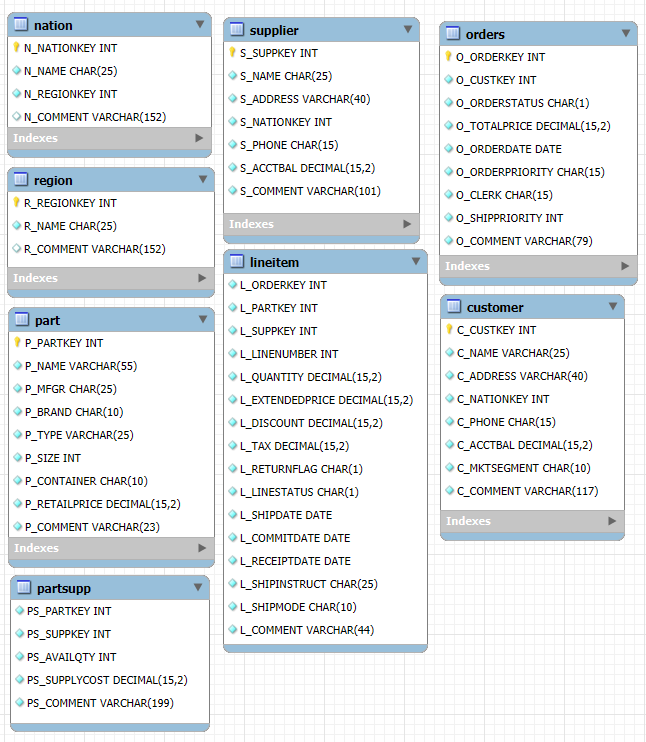
\includegraphics[width=0.75\linewidth]{img/image.png}
    \caption{Database Schema}
    \label{fig:database_schema}
\end{figure}


\chapter{Optimization Stages and Rule Application}
\thispagestyle{fancy}
The optimizer starts with the initial logical expression, which is a representation of the SQL query. This expression is then transformed through a series of stages, each applying a set of rules to optimize the query. \\
There are three main stages, each with its own set of rules and an unknown number of iterations, in order to target specific inefficiencies and improve the overall performance of the query execution plan. 

Throughout this report, we will refer to the initial state of the expression as \textbf{stage 0}, since it is the state before any optimization has been applied.
Below is a summary of the three stages and their respective rules:

\section{Stage 1: Pushdown Apply and Join Transformation}
In the first stage, the optimizer focuses on simplifying logical expressions and transforming subqueries into joins. The main goals are to:
\begin{itemize}
    \item \textbf{Simplify Boolean Expressions:} Rules such as \texttt{and\_rules} are used to simplify and normalize logical AND expressions, making the query plan easier to optimize in later stages.
    \item \textbf{Apply Always---Better Transformations:} The \texttt{always\_better\_rules} group contains general-purpose rules that are always beneficial, such as removing redundant operations or simplifying expressions.
    \item \textbf{Subquery to Join Conversion:} The \texttt{subquery\_rules} transform certain subqueries into equivalent join operations, enabling further optimizations and improving execution efficiency.
\end{itemize}

\section{Stage 2: Predicate and Projection Pushdown, Index Scan}
The second stage aims to reduce the amount of data processed by pushing filters and projections as close as possible to the data sources. The rules applied include:
\begin{itemize}
    \item \textbf{Expression Simplification:} General expression simplification rules (\texttt{expr::rules}) are applied to further normalize and reduce expressions.
    \item \textbf{Predicate Pushdown:} The \texttt{predicate\_pushdown\_rules} move filter conditions (WHERE clauses) down the query tree, so that irrelevant rows are filtered out early.
    \item \textbf{Projection Pushdown:} The \texttt{projection\_pushdown\_rules} ensure that only necessary columns are carried through each stage, minimizing data movement.
    \item \textbf{Index Scan Optimization:} The \texttt{index\_scan\_rules} attempt to replace full table scans with index scans when possible, improving query performance.
    \item \textbf{Always-Better Transformations:} These are re-applied to catch any new opportunities created by the previous rules.
\end{itemize}

\section{Stage 3: Join Reordering and Hash Join}
The third stage focuses on optimizing join operations, which are often the most expensive part of query execution. The rules in this stage include:
\begin{itemize}
    \item \textbf{Join Reordering:} The \texttt{join\_reorder\_rules} change the order in which joins are performed, aiming to minimize intermediate result sizes and overall cost.
    \item \textbf{Hash Join Optimization:} The \texttt{hash\_join\_rules} convert suitable joins into hash joins, which are more efficient for large datasets.
    \item \textbf{Predicate and Projection Pushdown:} These rules are re-applied to ensure that any new opportunities for pushdown created by join reordering are exploited.
    \item \textbf{Order Optimization:} The \texttt{order\_rules} optimize ORDER BY operations, potentially reducing sorting costs.
    \item \textbf{Boolean Simplification and Always-Better Transformations:} These are applied again to further refine the plan.
\end{itemize}

\subsection{Iterative Application}
Each group of rules is applied iteratively within its stage. The optimizer may revisit the same rule multiple times as the query plan evolves, ensuring that all possible optimizations are explored before moving to the next stage.


\chapter{Visual Representation and Analysis} \label{chap:concDesenho}
\thispagestyle{fancy}
The goal of the optimizer is mainly to reduce the cost of the execution of certain queries, this is accomplished through a series of optimization stages that eventually lead to a more efficient database. \\
Since our goal is to analyse this optimizer, we decided we should choose the TPC-H queries for which the cost decrease would be more significant. \\

We thought it would be helpful if we could see the cost for every query and compare it, before choosing the ones to further analyse. With this in mind and making use of the \textbf{Matplotlib library} in \textbf{Python}, we built a histogram, in which is displayed the cost for every stage the optimizer goes through. \\

The initial cost is omitted from this histogram, as it remains identical across all queries.
This value is defined as the maximum possible value that can be represented by a 32-bit floating point number and it is assigned using the line \textbf{\texttt{[let mut cost = f32::MAX]}}. This number has a value of approximately $3.4 \times 10^{38}$.

\begin{figure}[H]
    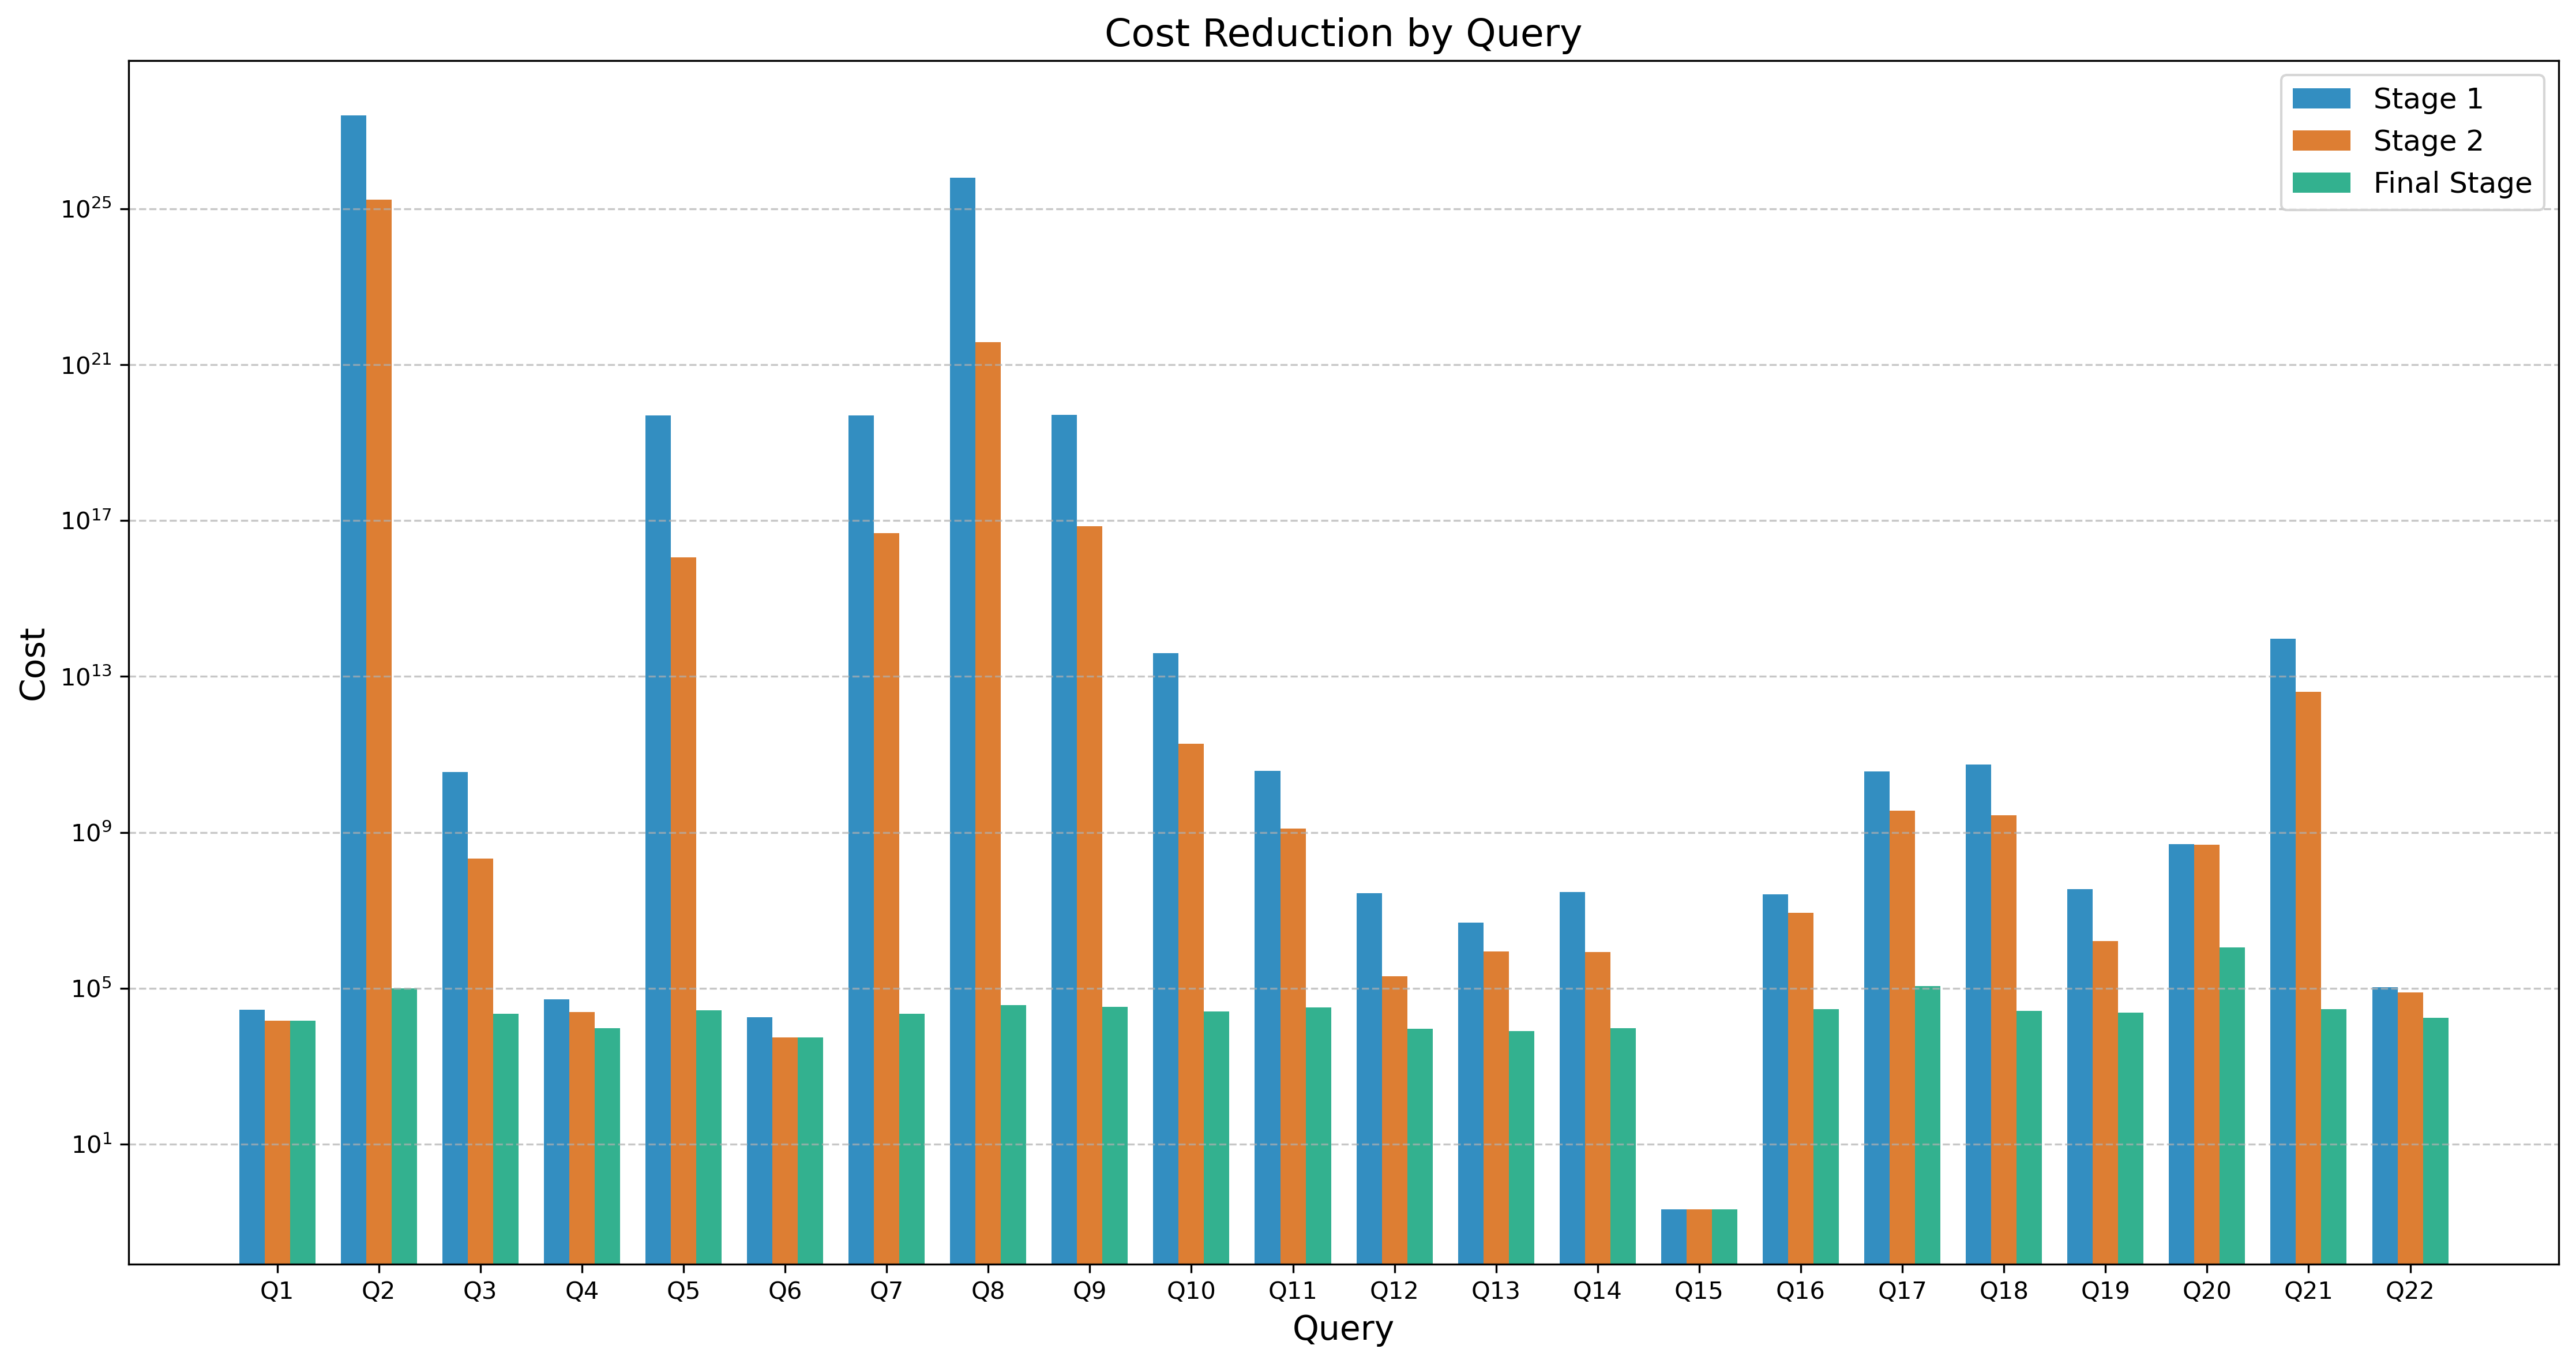
\includegraphics[width = 1.35\textwidth, height = 0.37\textheight, keepaspectratio]{img_cost_differential/cost_reduction_all_queries.png}
    \caption{Histogram of cost reduction}
    \label{fig:cost1}
\end{figure}

The histogram above does a good job at providing some insight as to what queries would be more advantageous to analyse with more depth. \\

To help understand the motivations behind this analysis, the table below has more detailed information about every query: initial and decreased costs alongside the stages.

\begin{figure}[H]
    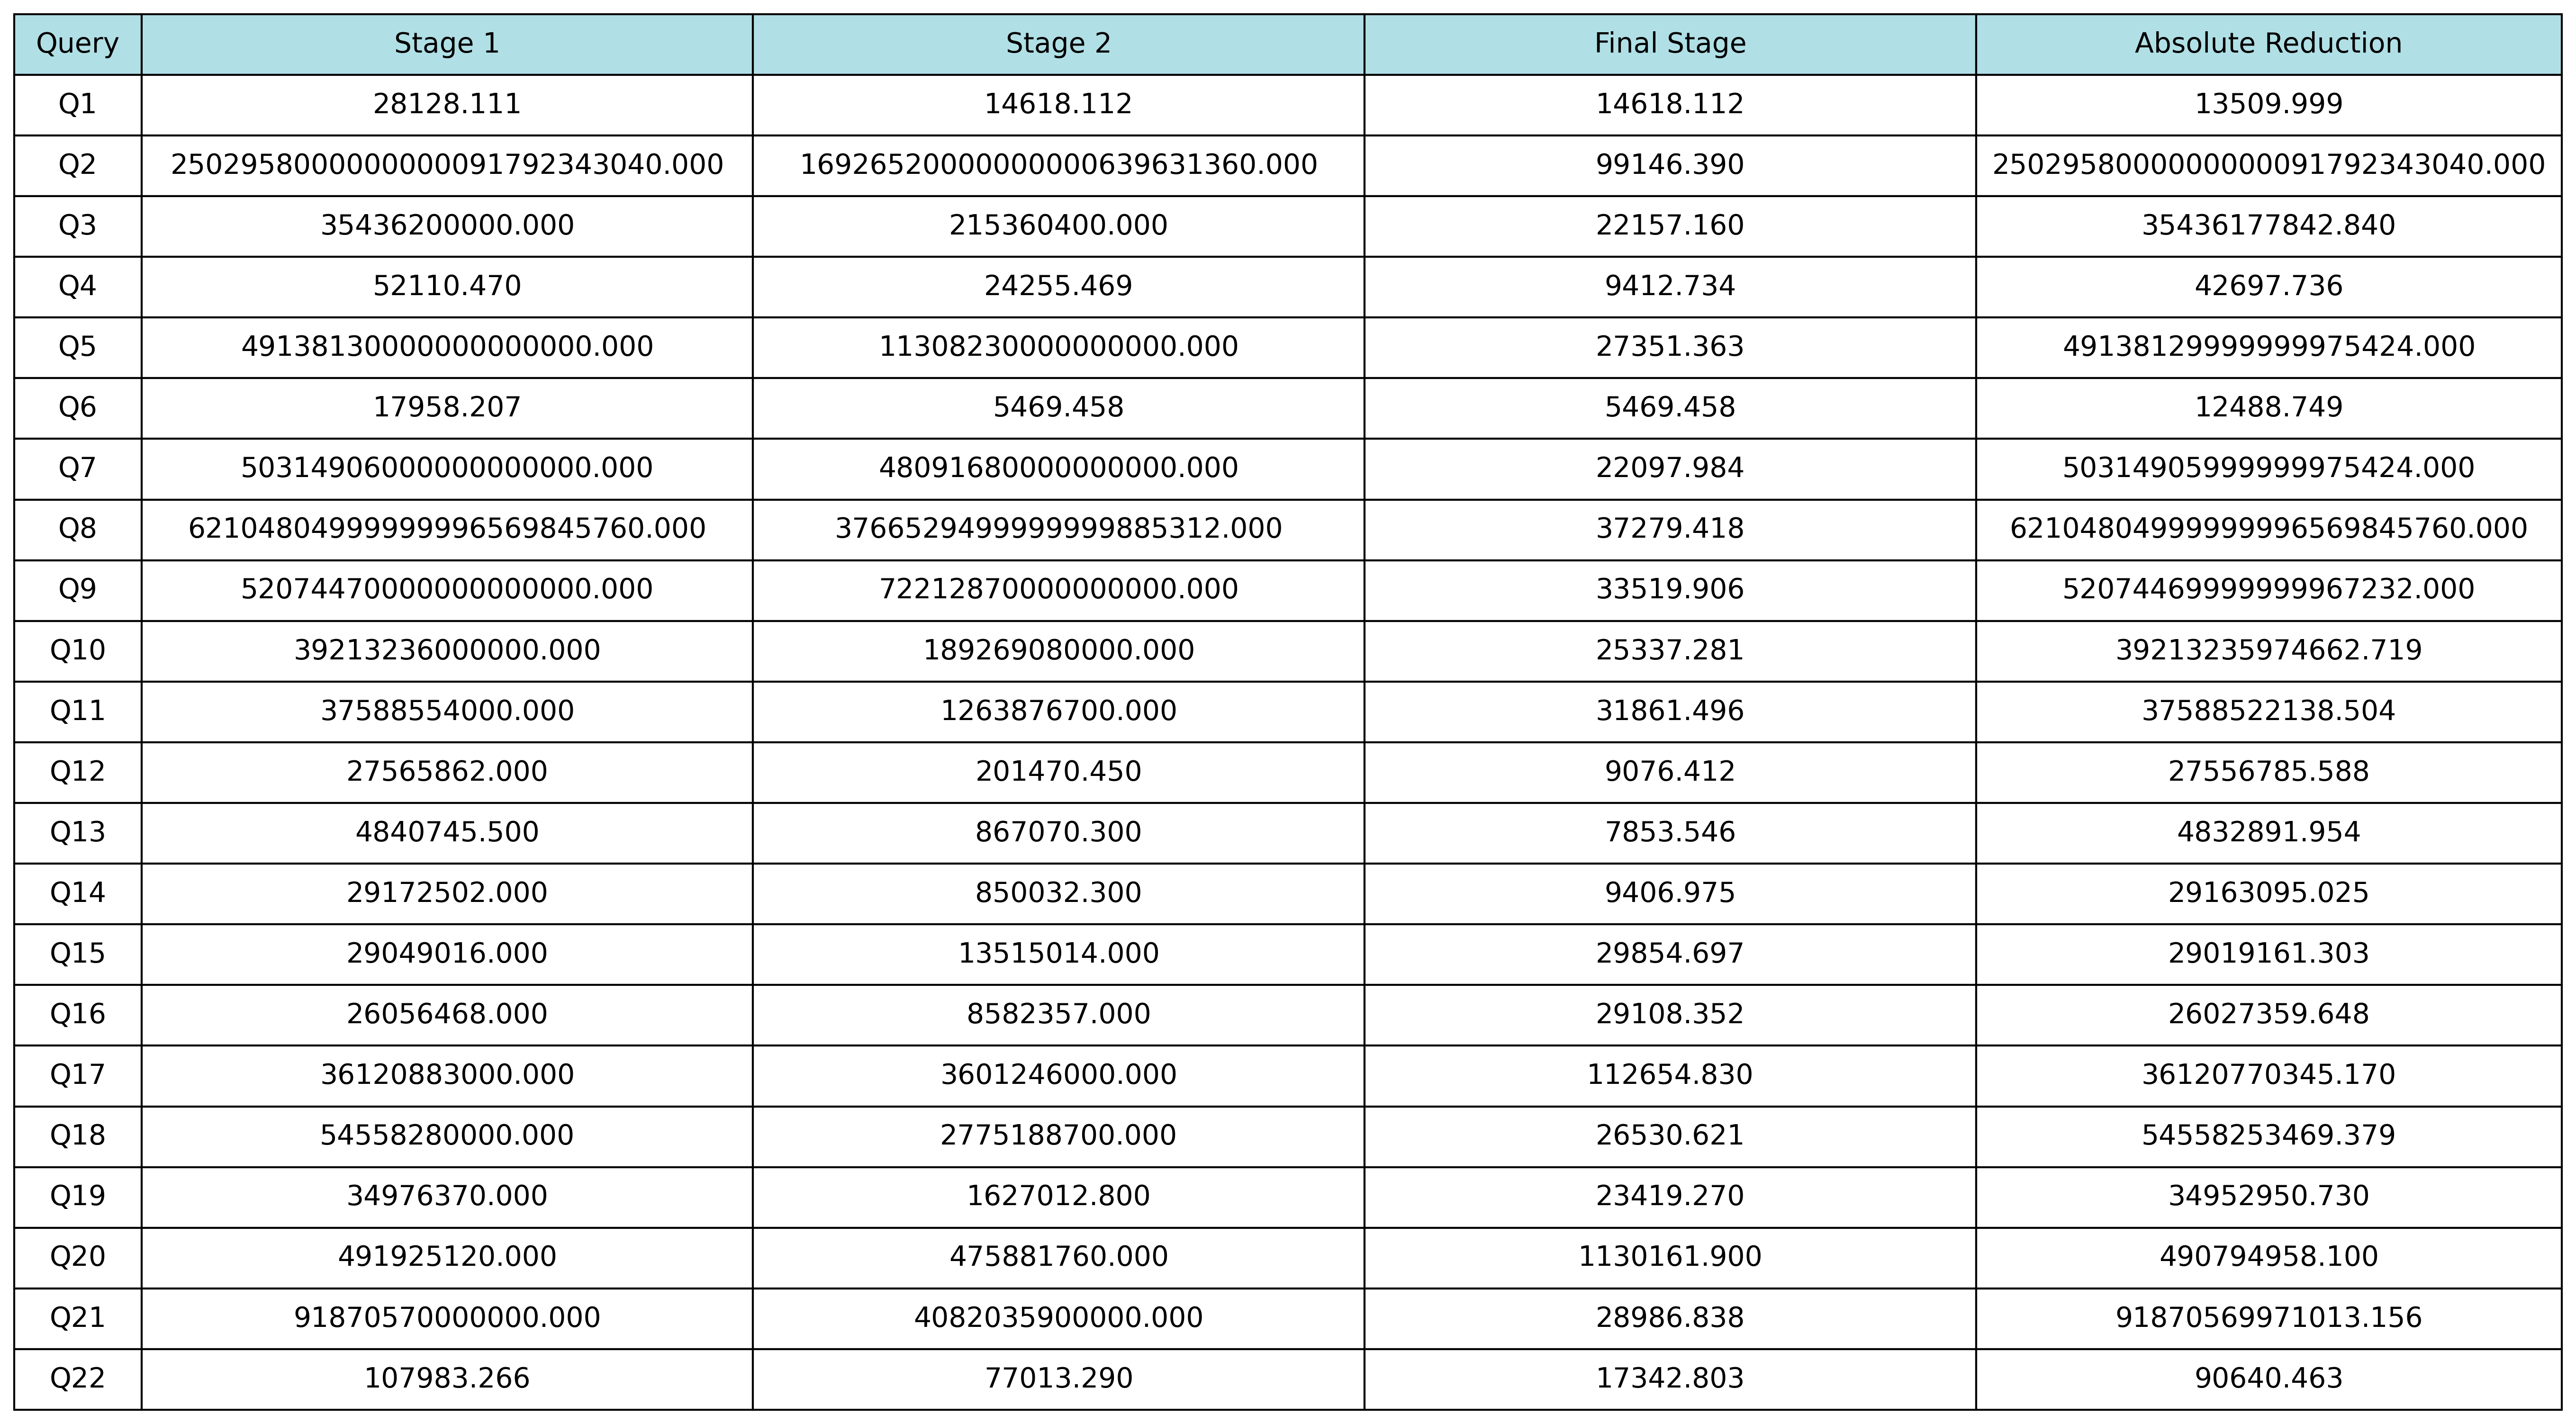
\includegraphics[width = 1.45\textwidth, height = 0.40\textheight, keepaspectratio]{img_cost_differential/cost_reduction_table.png}
    \caption{Table of cost reduction}
    \label{fig:tab1}
\end{figure}

As we can see in the images above, the cost decrease through the 3 stages is more accentuated in the queries 2, 5, 7, 8 and 9. We will look at these 5 queries more closely to get some more information about what causes the cost to decrease as much.\\

We found the accentuated decrease in cost more interesting, and this section will help understand the reasons behind it. \\

While this analysis is only focused on the 5 queries mentioned, the remaining queries' analysis will be available on our GitHub repository - \textbf{\href{https://github.com/Blackparkd/risinglight/tree/main/src/planner/outputs/graphs}{Graphs folder}} for the reader to explore. \\

First, for clarity purposes, we will display the query in SQL, next the relational expression generated, and only afterwards will we proceed with the in-depth analysis.

\section{Query 2}

\begin{lstlisting}
select
    s_acctbal,
    s_name,
    n_name,
    p_partkey,
    p_mfgr,
    s_address,
    s_phone,
    s_comment
from
    part,
    supplier,
    partsupp,
    nation,
    region
where
    p_partkey = ps_partkey
    and s_suppkey = ps_suppkey
    and p_size = 15
    and p_type like '%BRASS'
    and s_nationkey = n_nationkey
    and n_regionkey = r_regionkey
    and r_name = 'EUROPE'
    and ps_supplycost = (
        select
            min(ps_supplycost)
        from
            partsupp,
            supplier,
            nation,
            region
        where
            p_partkey = ps_partkey
            and s_suppkey = ps_suppkey
            and s_nationkey = n_nationkey
            and n_regionkey = r_regionkey
            and r_name = 'EUROPE'
    )
order by
    s_acctbal desc,
    n_name,
    s_name,
    p_partkey
limit 100;
\end{lstlisting}

\subsubsection{Relational Expression}

The relational expression is a representation of the SQL query in a tree-like structure, where each node represents an operation or a relation. The expression is generated by the optimizer and serves as an intermediate representation before the final execution plan is created.

\textbf{Stage 0:}

\begin{exprlisting}
RecExpr { nodes: [Constant(Bool(true)), Column($1.2(1)), Column($1.1(1)), Column($1.0(1)), List([3, 2, 1]), Table($1), Scan([5, 4, 0]), Column($0.3(1)), Column($0.2(1)), Column($0.1(1)), Column($0.0(1)), List([10, 9, 8, 7]), Table($0), Scan([12, 11, 0]), Column($3.6(1)), Column($3.5(1)), Column($3.4(1)), Column($3.3(1)), Column($3.2(1)), Column($3.1(1)), Column($3.0(1)), List([20, 19, 18, 17, 16, 15, 14]), Table($3), Scan([22, 21, 0]), Column($4.4(1)), Column($4.3(1)), Column($4.2(1)), Column($4.1(1)), Column($4.0(1)), List([28, 27, 26, 25, 24]), Table($4), Scan([30, 29, 0]), Inner, Join([32, 0, 31, 23]), Join([32, 0, 33, 13]), Join([32, 0, 34, 6]), Constant(String(""EUROPE"")), Eq([2, 36]), Eq([8, 3]), Eq([17, 10]), Eq([20, 27]), Column($2.0), Eq([41, 28]), And([42, 40]), And([43, 39]), And([44, 38]), And([45, 37]), Filter([46, 35]), Min(25), List([48]), Agg([49, 47]), Filter([0, 50]), List([]), Order([52, 51]), Ref(48), List([54]), Proj([55, 53]), Constant(Int32(0)), Constant(Null), Limit([58, 57, 56]), Column($1.2), Column($1.1), Column($1.0), List([62, 61, 60]), Scan([5, 63, 0]), Column($0.3), Column($0.2), Column($0.1), Column($0.0), List([68, 67, 66, 65]), Scan([12, 69, 0]), Column($4.4), Column($4.3), Column($4.2), Column($4.1), Column($4.0), List([75, 74, 73, 72, 71]), Scan([30, 76, 0]), Column($3.6), Column($3.5), Column($3.4), Column($3.3), Column($3.2), Column($3.1), Column($3.0), List([84, 83, 82, 81, 80, 79, 78]), Scan([22, 85, 0]), Column($2.8), Column($2.7), Column($2.6), Column($2.5), Column($2.4), Column($2.3), Column($2.2), Column($2.1), List([41, 94, 93, 92, 91, 90, 89, 88, 87]), Table($2), Scan([96, 95, 0]), Join([32, 0, 97, 86]), Join([32, 0, 98, 77]), Join([32, 0, 99, 70]), Join([32, 0, 100, 64]), LeftOuter, Apply([102, 101, 59]), Eq([72, 54]), Eq([61, 36]), Eq([66, 62]), Eq([81, 68]), Constant(String(""\%BRASS"")), Like([91, 108]), Constant(Int32(15)), Eq([90, 110]), Eq([84, 74]), Eq([41, 75]), And([113, 112]), And([114, 111]), And([115, 109]), And([116, 107]), And([117, 106]), And([118, 105]), And([119, 104]), Filter([120, 103]), Filter([0, 121]), Desc(79), List([123, 67, 83, 41]), Order([124, 122]), List([79, 83, 67, 41, 93, 82, 80, 78]), Proj([126, 125]), Constant(Int32(100)), Limit([128, 57, 127])] }
\end{exprlisting}

One more reason to show the stage 0 expression is to show how the optimizer starts with a very complex expression (containing 129 nodes), and how it is gradually simplified throughout the stages. \\

\textbf{Stage 3:}

\begin{exprlisting}
RecExpr { nodes: [Constant(Bool(true)), Column($4.3(1)), Column($4.1(1)), Column($4.0(1)), List([3, 2, 1]), Table($4), Scan([5, 4, 0]), Column($3.3(1)), Column($3.0(1)), List([8, 7]), Table($3), Scan([10, 9, 0]), Column($0.2(1)), Column($0.0(1)), List([13, 12]), Table($0), Scan([15, 14, 0]), Column($1.1(1)), Column($1.0(1)), List([18, 17]), Table($1), Scan([20, 19, 0]), Constant(String(""EUROPE"")), Eq([17, 22]), Filter([23, 21]), List([18]), Proj([25, 24]), List([12]), Inner, HashJoin([28, 0, 25, 27, 26, 16]), List([13]), Proj([30, 29]), List([7]), HashJoin([28, 0, 30, 32, 31, 11]), List([8]), Proj([34, 33]), List([2]), HashJoin([28, 0, 34, 36, 35, 6]), List([3, 1]), Proj([38, 37]), Column($4.4), Column($4.3), Column($4.2), Column($4.1), Column($4.0), List([44, 43, 42, 41, 40]), Scan([5, 45, 0]), Column($3.6), Column($3.5), Column($3.4), Column($3.3), Column($3.2), Column($3.1), Column($3.0), List([53, 52, 51, 50, 49, 48, 47]), Scan([10, 54, 0]), Column($1.2), Column($1.1), Column($1.0), List([58, 57, 56]), Scan([20, 59, 0]), Eq([22, 57]), Filter([61, 60]), Column($0.3), Column($0.2), Column($0.1), Column($0.0), List([66, 65, 64, 63]), Scan([15, 67, 0]), List([58]), List([64]), HashJoin([28, 0, 70, 69, 68, 62]), List([50]), List([66]), HashJoin([28, 0, 73, 72, 71, 55]), List([43]), List([53]), HashJoin([28, 0, 76, 75, 74, 46]), List([53, 52, 51, 50, 49, 48, 47, 44, 43, 42, 41, 40, 66, 65, 64, 63, 58, 57, 56]), Proj([78, 77]), Column($2.8), Column($2.7), Column($2.6), Column($2.5), Column($2.4), Column($2.3), Column($2.2), Column($2.1), Column($2.0), List([88, 87, 86, 85, 84, 83, 82, 81, 80]), Table($2), Scan([90, 89, 0]), Constant(Int32(15)), Eq([83, 92]), Constant(String(""\%BRASS"")), Like([84, 94]), And([95, 93]), Filter([96, 91]), List([44]), List([88]), HashJoin([28, 0, 99, 98, 97, 79]), List([3]), LeftOuter, HashJoin([102, 0, 99, 98, 97, 79]), List([3]), Proj([106, 105]), Constant(Int32(100)), Limit([108, 57, 107])] }
\end{exprlisting}

As we can see, the optimizer managed to reduce the number of nodes from 129 in the initial expression to 109 in the final optimized form, while maintaining the semantic equivalence of the query. \\ This reduction in complexity is one of the factors that contributes to the overall cost decrease. \\

So now, a good question to ask is: \textbf{How does the optimizer manage to reduce the number of nodes?} \\

To help answering this question, it is helpful to analyse the histogram of the expression groups generated during the optimization process. 

\subsection{Expression Groups}

The expression groups are a representation of the different equivalent expressions generated during the optimization process. Each group contains expressions that are semantically equivalent but may differ in their internal representation. \\

\begin{figure}[H]
    \centering
    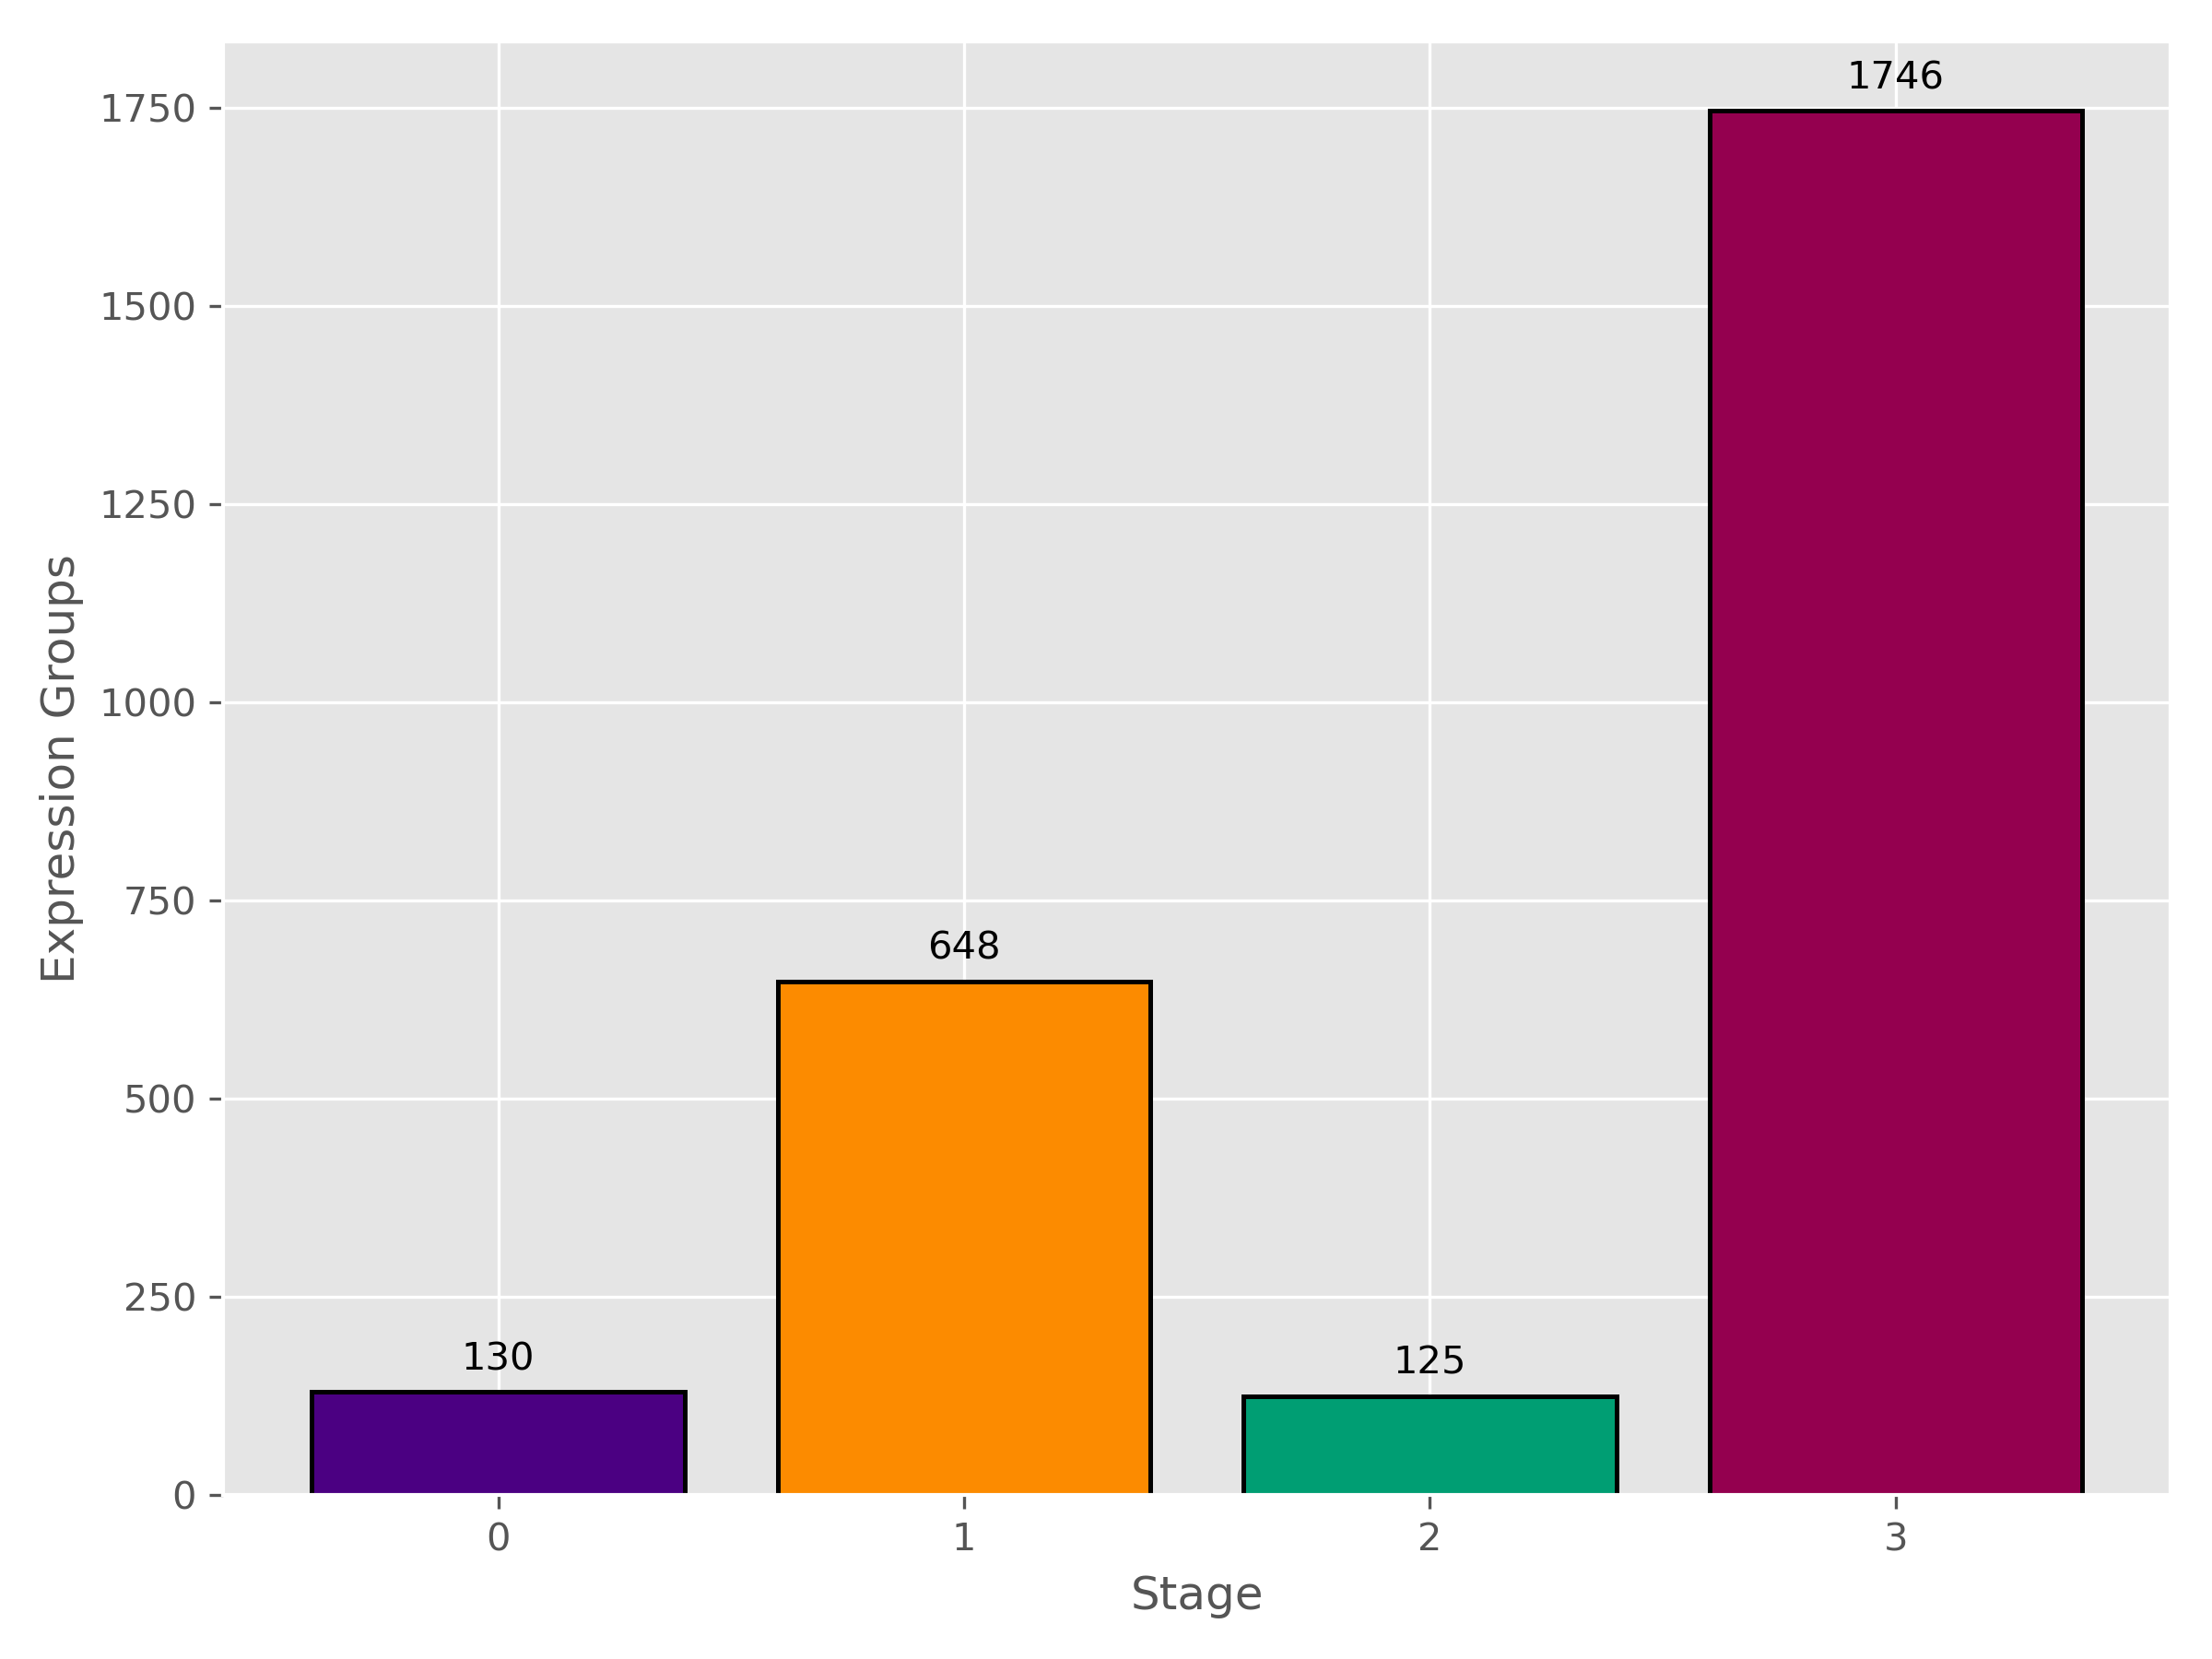
\includegraphics[width=0.80\linewidth]{img/expression_groups/q2_expression_groups.png}
    \caption{Query 2 - Expression Groups}
    \label{fig:exprgroups2}
\end{figure}

The histogram above displays the number of expression groups generated at each stage of the optimization process. Within each group, there may be an unknown number of equivalent expressions. \\

According to the \textbf{Cost Reduction} histogram (Figure \ref{fig:cost1}), the decrease in cost is more accentuated when we move from stage 2 to stage 3. This is the stage where the optimizer applies the join reordering and hash join rules. \\
This is also reflected in the histogram of expression groups (Figure \ref{fig:exprgroups2}), where we can see that the number of groups generated in stage 3 is significantly higher than in stage 2. \\
This gives the impression that the optimizer is, not only exploring a larger number of equivalent expressions in stage 3, but also being able to reduce the overall cost of the query. \\

This is a very interesting finding, as it suggests that the optimizer is capable of finding more efficient ways to represent the same operation, even when the number of equivalent expressions increases. \\

\subsection{Rule Application}

Given these new results, we can't help but wonder what exactly is happening during this stage that might trigger this increase in the number of expression groups. \\ Looking at the code in the \texttt{optimizer.rs} file, it's possible to learn exactly what rules are being applied during this stage. \\

The rules are defined in the \texttt{src/planner/rules} folder, and they are grouped into different categories. The rules that are applied during stage 3 are defined in the \texttt{src/planner/rules/plan.rs} file. \\

\begin{lstlisting}[language=Rust]
static STAGE3_RULES: LazyLock<Vec<Rewrite>> = LazyLock::new(|| {
    let mut rules = vec![];
    rules.append(&mut rules::expr::and_rules());
    rules.append(&mut rules::plan::always_better_rules());
    rules.append(&mut rules::plan::join_reorder_rules());
    rules.append(&mut rules::plan::hash_join_rules());
    rules.append(&mut rules::plan::predicate_pushdown_rules());
    rules.append(&mut rules::plan::projection_pushdown_rules());
    rules.append(&mut rules::order::order_rules());
    rules
});
\end{lstlisting}

\begin{figure}[H]
    \centering
    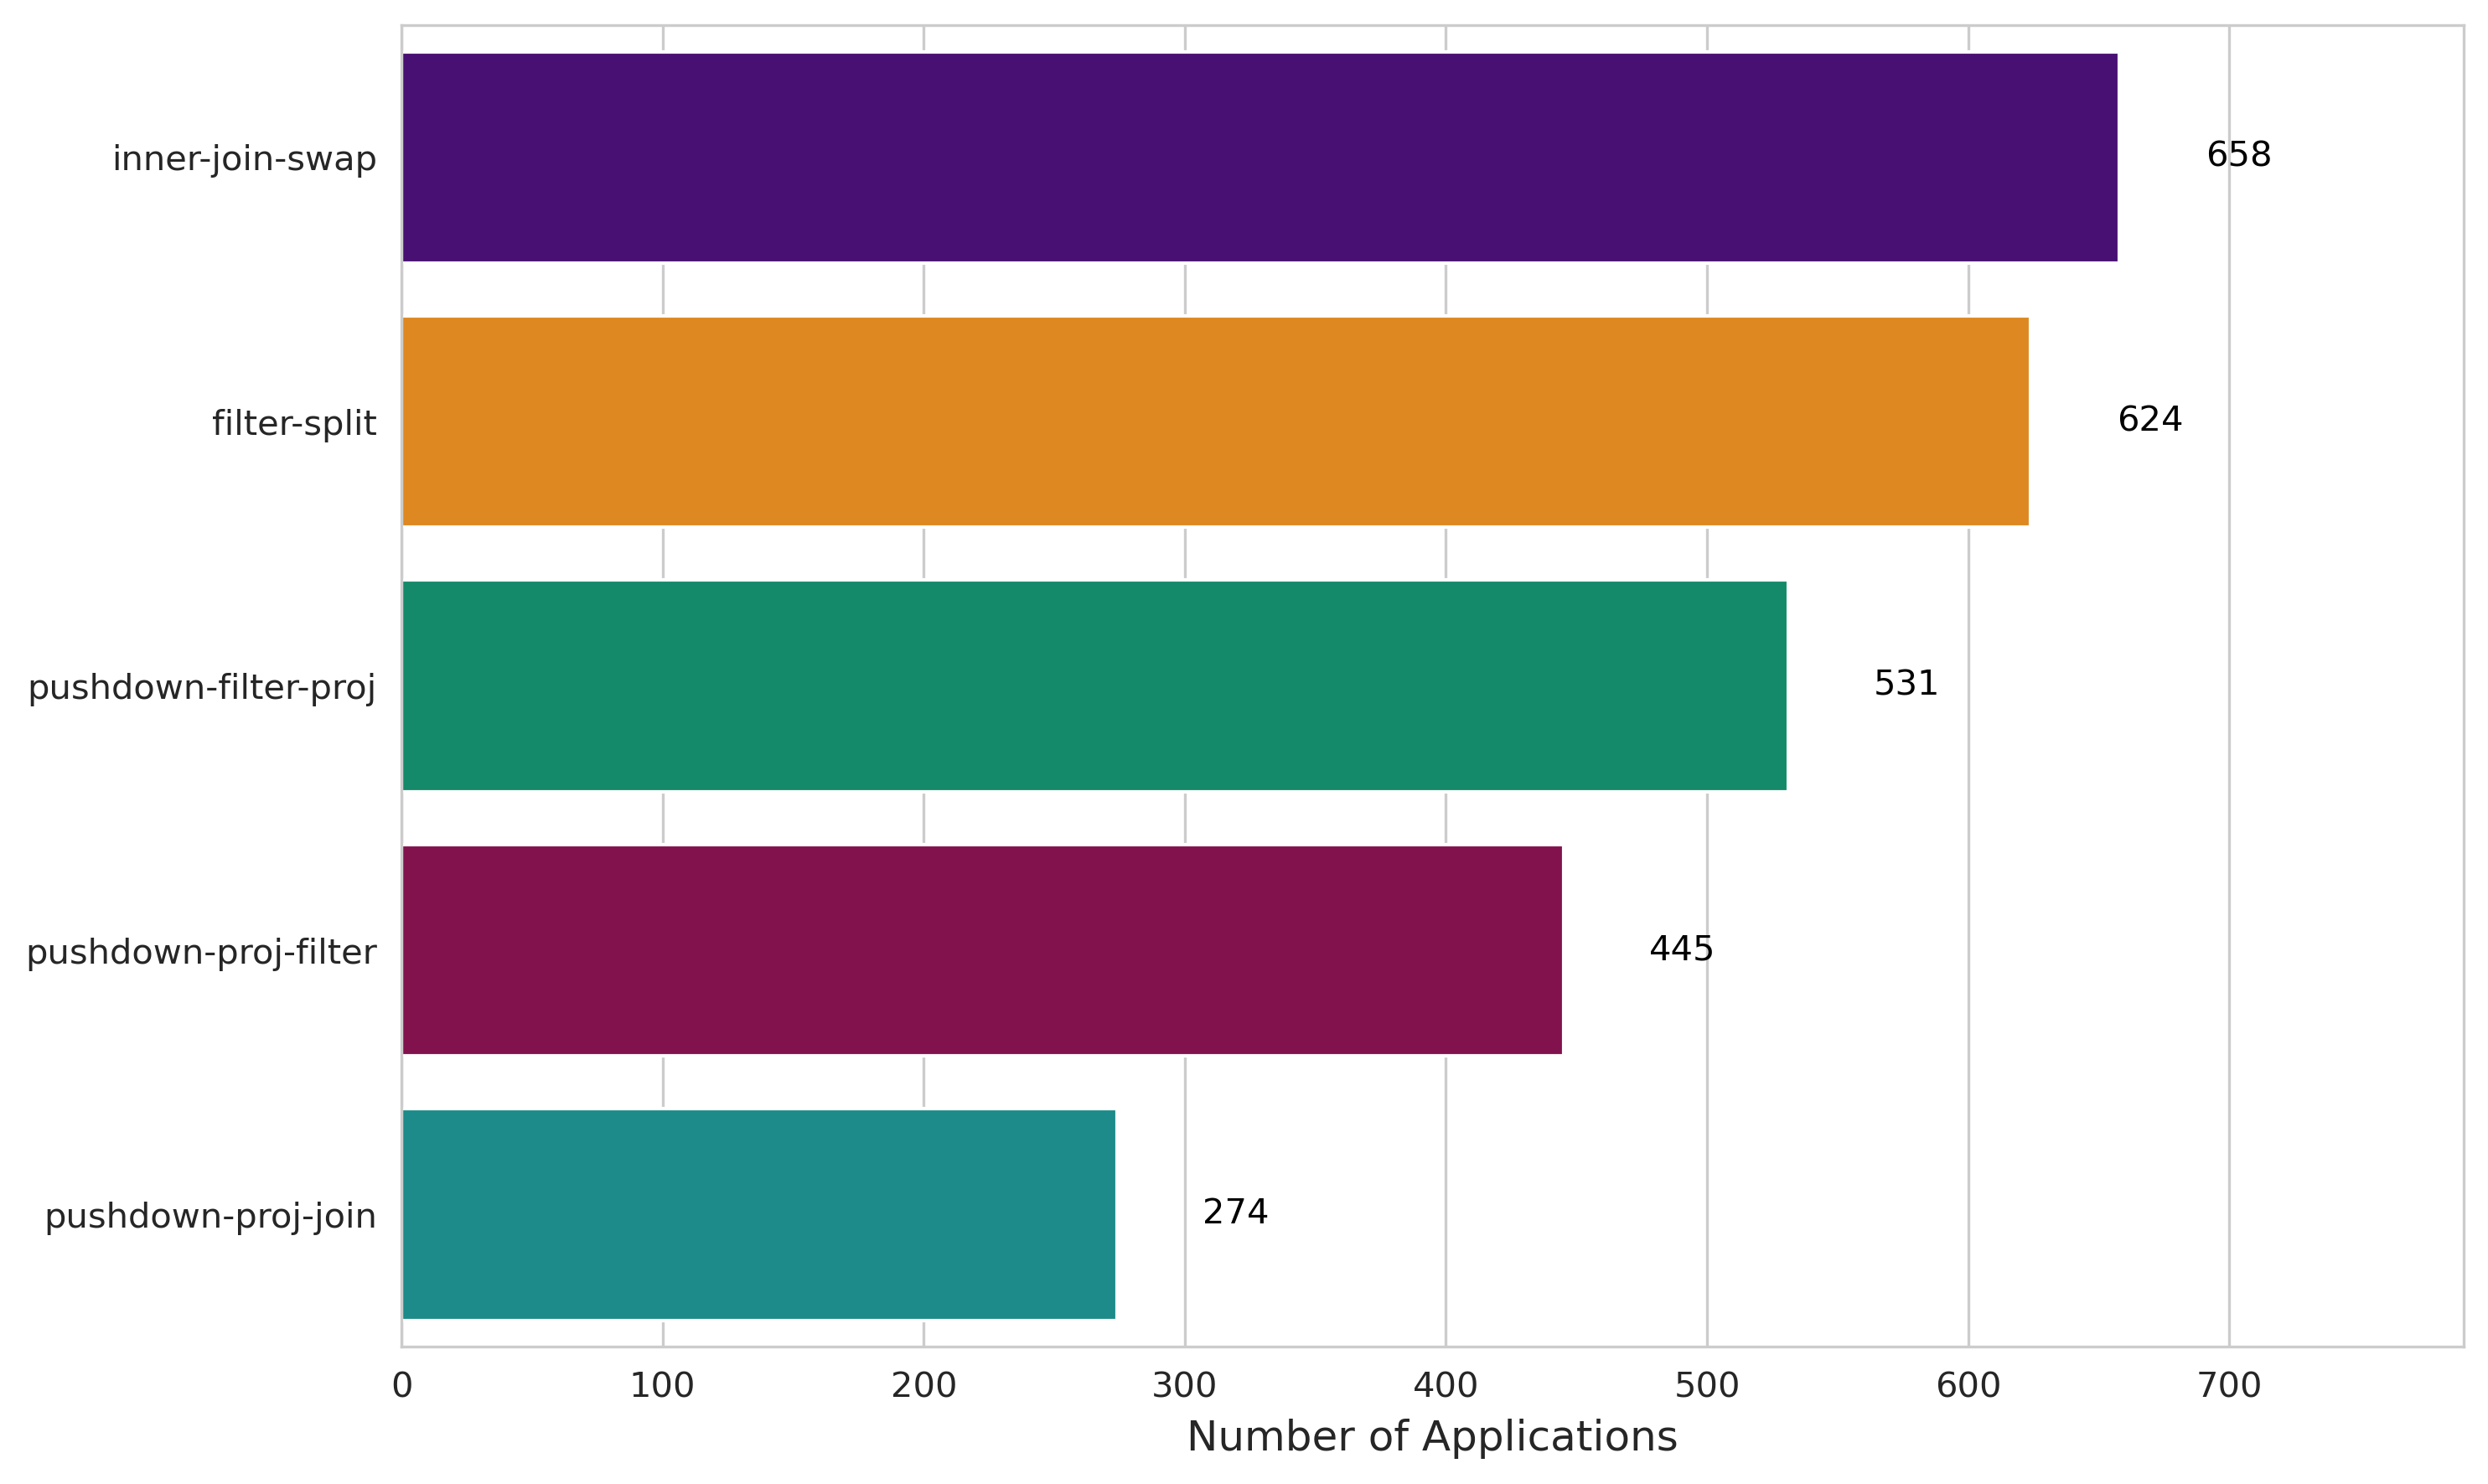
\includegraphics[width=0.95\linewidth]{img/img_rule_mostpop/top_5_rules_stage3_q2.png}
    \caption{Query 2 - Rules in Stage 3}
    \label{fig:rules2}
\end{figure}

Looking at the most popular rules applied during stage 3 (Figure \ref{fig:rules2}), we can see that the most frequently applied rules are related to join operations and projection pushdown. This aligns with our understanding that stage 3 focuses heavily on optimizing joins and their order of execution.

The high frequency of join-related rule applications explains the increase in expression groups, as each new join order or implementation strategy generates new equivalent expressions. Despite this increase in complexity, the optimizer successfully reduces the query's cost through these transformations.

A rule \texttt{inner-join-swap} being the most frequently applied shows how significant join reordering is for query optimization. \\

Consider the basic associativity transformation: $(A \bowtie B) \bowtie C \Rightarrow A \bowtie (B \bowtie C)$. This seemingly simple change in join order can drastically impact performance. If table $B \bowtie C$ produces a smaller intermediate result than $A \bowtie B$, the right-side expression requires less memory and computation in subsequent joins. \\
This transformation alone was applied 658 times during stage 3 optimization of Query 2, suggesting how extensively the optimizer explores the space of possible join orders to find the most efficient execution plan.

\subsection{Merge Operations}


During stage 3, the optimizer applies join reordering rules and other transformations that generate a large number of new equivalent expressions. Each new join order or execution strategy can result in different representations for the same logical operation. As a consequence, the number of expression groups grows rapidly. \\
However, many of these new expressions end up being semantically equivalent to each other. The merge mechanism of the optimizer serves precisely to identify and merge these equivalent expressions into a single group, reducing redundancy in the e-graph. Therefore, a significant increase in the number of merge operations is expected at this stage, reflecting the intense exploration of execution plan space and the subsequent consolidation of equivalent expressions.


\begin{figure}[H]
    \centering
    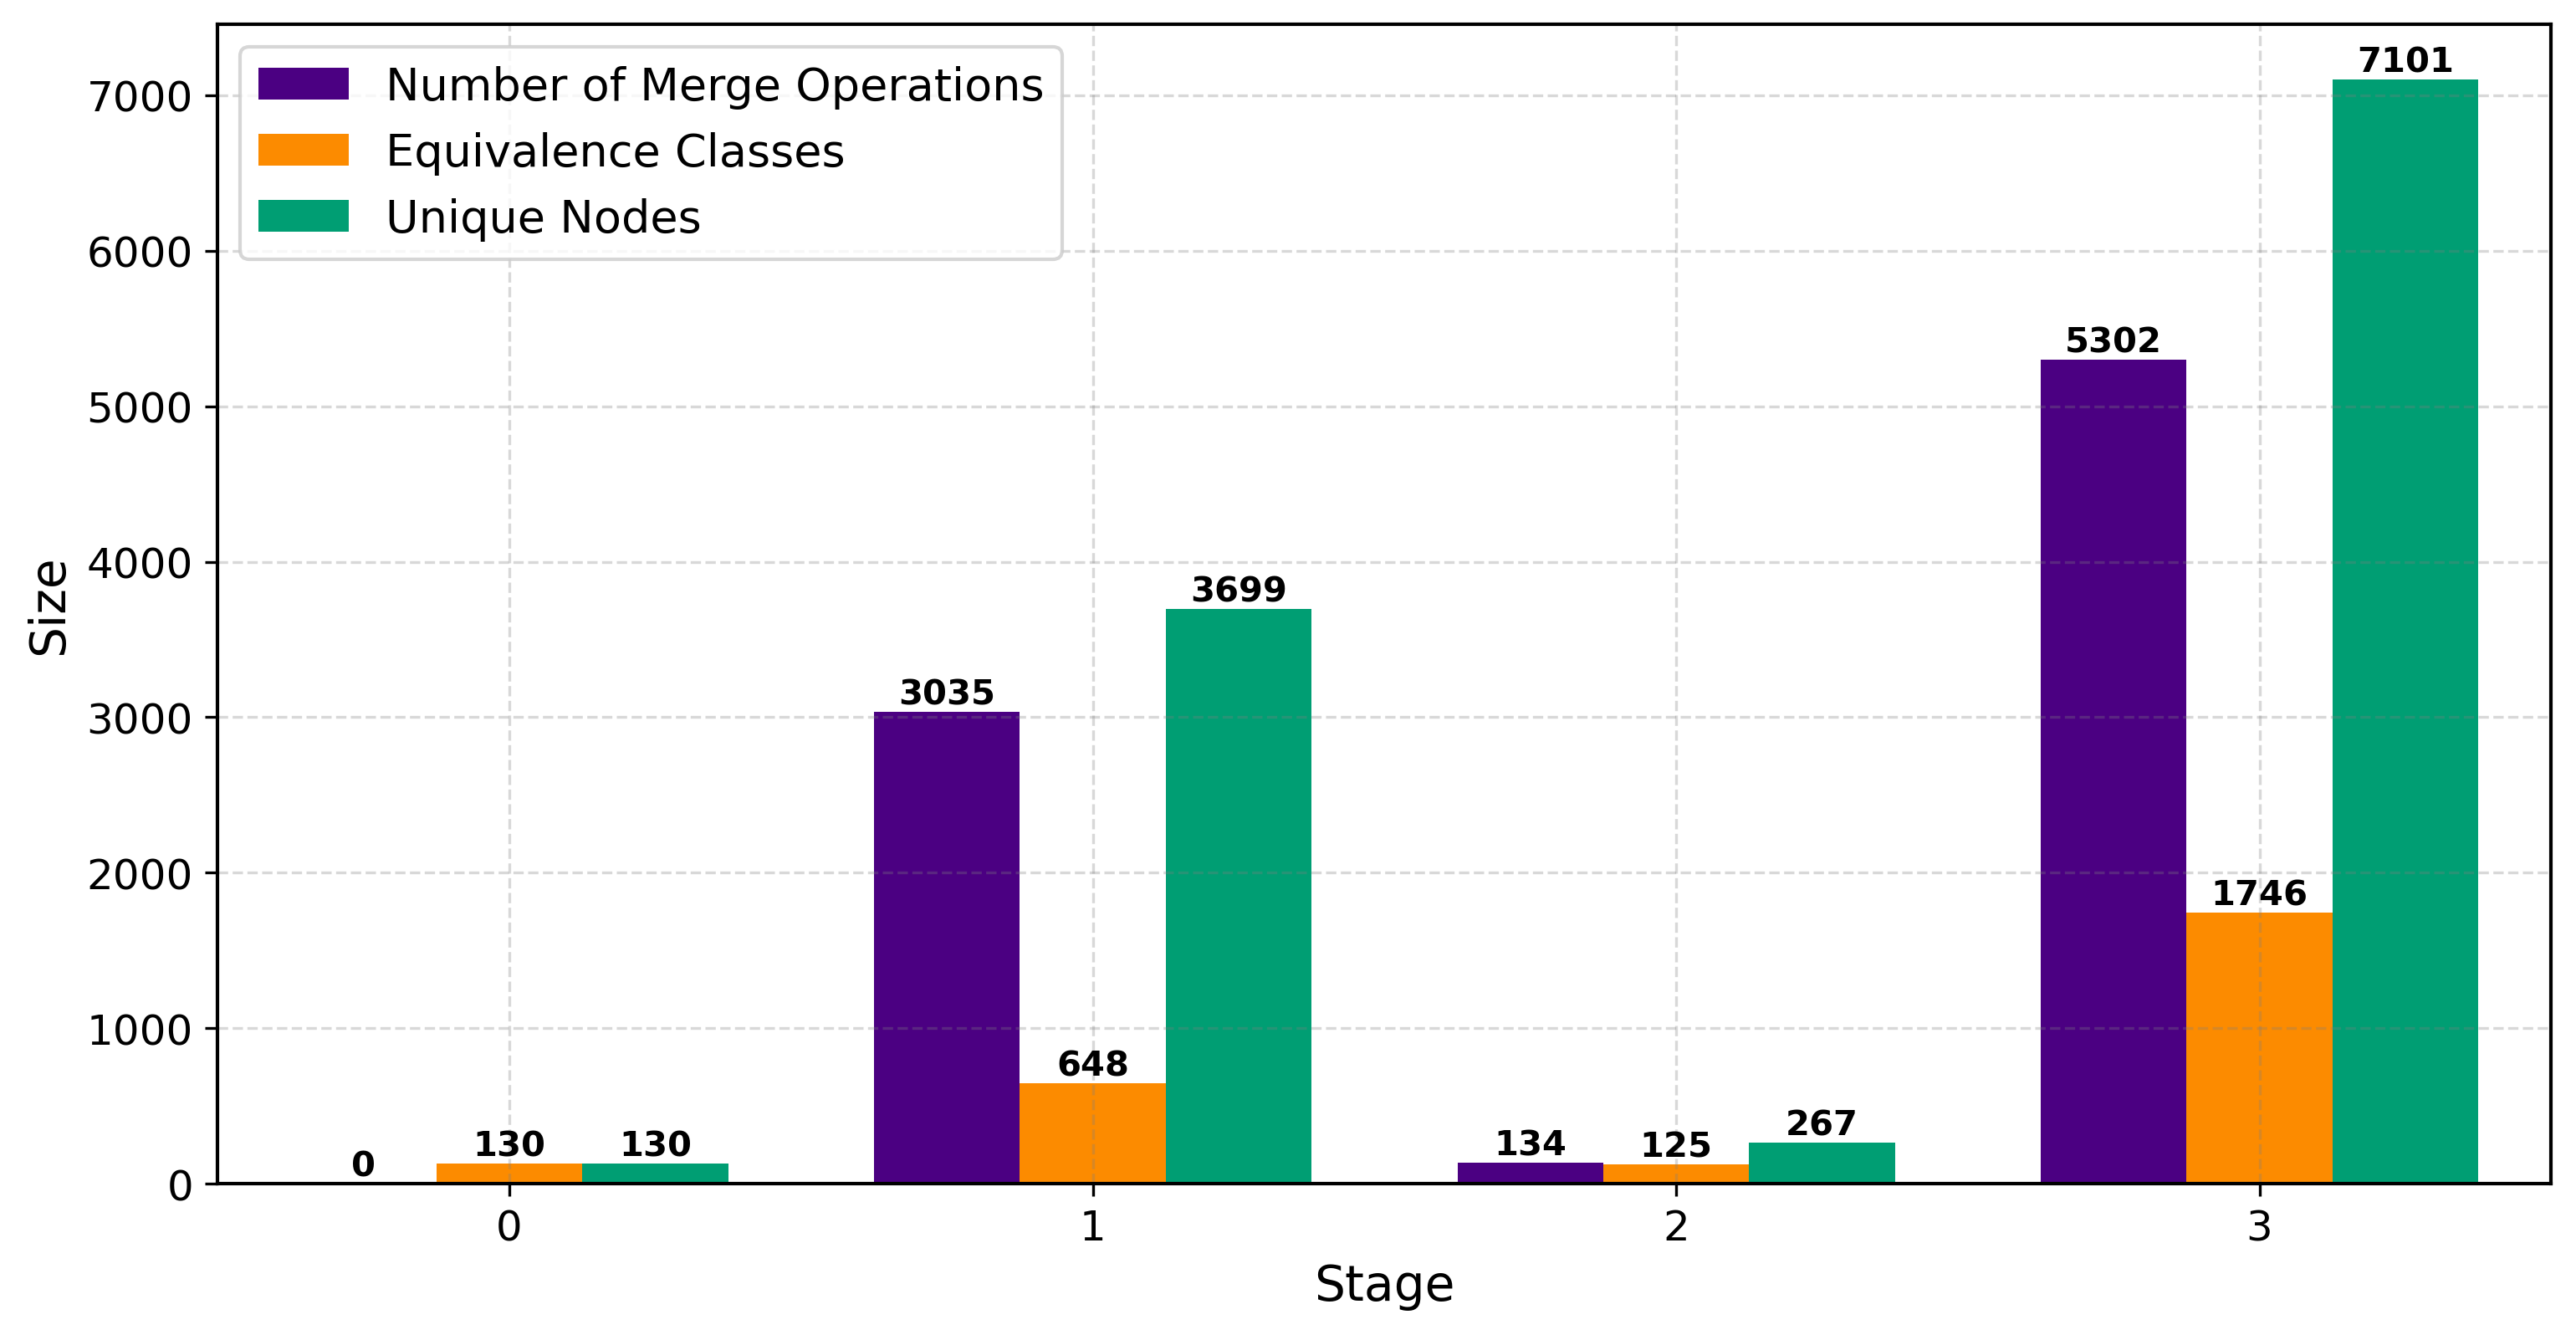
\includegraphics[width=\linewidth]{img_merges/q2_sizes.png}
    \caption{Query 2 - Merge operations}
    \label{fig:hist2}
\end{figure}

Here we can see that the optimizer has the expected behavior: The number of merge operations greatly increases, which means that, despite the increase in the number of expression groups generated during stage 3, a large group of these are also being merged into a single representation. \\

This histogram also has some interesting information about the number of equivalence classes and the number of unique nodes. Each equivalence class represents a group in which all the expressions are equivalent, while each node is an unique expression, for example, the expression \texttt{"a+b"} is a possible node.\\ 
However, \texttt{"b+a"} can also be a node, but since they represent the same operation, they can be merged into a single equivalence class. \\
This is the reason for the difference between the number of equivalence classes and the number of unique nodes, in stages where the growth of expression groups is more accentuated. \\

\section{Query 8}
\begin{lstlisting}
    select
    o_year,
    sum(case
        when nation = 'IRAQ' then volume
        else 0
    end) / sum(volume) as mkt_share
from
    (
        select
            extract(year from o_orderdate) as o_year,
            l_extendedprice * (1 - l_discount) as volume,
            n2.n_name as nation
        from
            part,
            supplier,
            lineitem,
            orders,
            customer,
            nation n1,
            nation n2,
            region
        where
            p_partkey = l_partkey
            and s_suppkey = l_suppkey
            and l_orderkey = o_orderkey
            and o_custkey = c_custkey
            and c_nationkey = n1.n_nationkey
            and n1.n_regionkey = r_regionkey
            and r_name = 'AMERICA'
            and s_nationkey = n2.n_nationkey
            and o_orderdate between date '1995-01-01' and date '1996-12-31'
            and p_type = 'ECONOMY ANODIZED STEEL'
    ) as all_nations
group by
    o_year
order by
    o_year;
\end{lstlisting}

\subsubsection{Relational Expression}
\textbf{Stage 0:}
\begin{exprlisting}
    "RecExpr { nodes: [Constant(Bool(true)), Column($1.2), Column($1.1), Column($1.0), List([3, 2, 1]), Table($1), Scan([5, 4, 0]), Column($0.3(1)), Column($0.2(1)), Column($0.1(1)), Column($0.0(1)), List([10, 9, 8, 7]), Table($0), Scan([12, 11, 0]), Column($0.3), Column($0.2), Column($0.1), Column($0.0), List([17, 16, 15, 14]), Scan([12, 18, 0]), Column($5.7), Column($5.6), Column($5.5), Column($5.4), Column($5.3), Column($5.2), Column($5.1), Column($5.0), List([27, 26, 25, 24, 23, 22, 21, 20]), Table($5), Scan([29, 28, 0]), Column($6.8), Column($6.7), Column($6.6), Column($6.5), Column($6.4), Column($6.3), Column($6.2), Column($6.1), Column($6.0), List([39, 38, 37, 36, 35, 34, 33, 32, 31]), Table($6), Scan([41, 40, 0]), Column($7.15), Column($7.14), Column($7.13), Column($7.12), Column($7.11), Column($7.10), Column($7.9), Column($7.8), Column($7.7), Column($7.6), Column($7.5), Column($7.4), Column($7.3), Column($7.2), Column($7.1), Column($7.0), List([58, 57, 56, 55, 54, 53, 52, 51, 50, 49, 48, 47, 46, 45, 44, 43]), Table($7), Scan([60, 59, 0]), Column($3.6), Column($3.5), Column($3.4), Column($3.3), Column($3.2), Column($3.1), Column($3.0), List([68, 67, 66, 65, 64, 63, 62]), Table($3), Scan([70, 69, 0]), Column($2.8), Column($2.7), Column($2.6), Column($2.5), Column($2.4), Column($2.3), Column($2.2), Column($2.1), Column($2.0), List([80, 79, 78, 77, 76, 75, 74, 73, 72]), Table($2), Scan([82, 81, 0]), Inner, Join([84, 0, 83, 71]), Join([84, 0, 85, 61]), Join([84, 0, 86, 42]), Join([84, 0, 87, 30]), Join([84, 0, 88, 19]), Join([84, 0, 89, 13]), Join([84, 0, 90, 6]), Constant(String(""ECONOMY ANODIZED STEEL"")), Eq([76, 92]), Constant(Date(Date(9861))), LtEq([35, 94]), Constant(Date(Date(9131))), GtEq([35, 96]), And([97, 95]), Eq([65, 10]), Constant(String(""AMERICA"")), Eq([2, 100]), Eq([15, 3]), Eq([24, 17]), Eq([38, 27]), Eq([58, 39]), Eq([68, 56]), Eq([80, 57]), And([107, 106]), And([108, 105]), And([109, 104]), And([110, 103]), And([111, 102]), And([112, 101]), And([113, 99]), And([114, 98]), And([115, 93]), Filter([116, 91]), Filter([0, 117]), List([]), Order([119, 118]), Constant(Int32(1)), Sub([121, 52]), Mul([53, 122]), Field(DateTimeField(Year)), Extract([124, 35]), List([125, 123, 9]), Proj([126, 120]), Constant(Int32(0)), Constant(Null), Limit([129, 128, 127]), Filter([0, 130]), Ref(123), Sum(132), Type(Decimal(Some(30), Some(4))), Cast([134, 128]), Constant(String(""IRAQ"")), Eq([9, 136]), If([137, 132, 135]), Sum(138), List([139, 133]), Ref(125), List([141]), HashAgg([142, 140, 131]), Filter([0, 143]), Order([142, 144]), Ref(133), Ref(139), Div([147, 146]), List([141, 148]), Proj([149, 145]), Limit([129, 128, 150])] }"
\end{exprlisting}

\textbf{Stage 3:}

\begin{exprlisting}
    "RecExpr { nodes: [Constant(Bool(true)), Column($0.2), Column($0.0), List([2, 1]), Table($0), Scan([4, 3, 0]), Column($2.4), Column($2.0), List([7, 6]), Table($2), Scan([9, 8, 0]), Constant(String(""ECONOMY ANODIZED STEEL"")), Eq([6, 11]), Filter([12, 10]), List([7]), Proj([14, 13]), Column($5.3), Column($5.0), List([17, 16]), Table($5), Scan([19, 18, 0]), Column($6.4), Column($6.1), Column($6.0), List([23, 22, 21]), Table($6), Scan([25, 24, 0]), Constant(Date(Date(9131))), GtEq([21, 27]), Constant(Date(Date(9861))), GtEq([29, 21]), And([30, 28]), Filter([31, 26]), List([17]), List([22]), Inner, HashJoin([35, 0, 34, 33, 32, 20]), List([23, 21, 16]), Proj([37, 36]), Column($7.6), Column($7.5), Column($7.2), Column($7.1), Column($7.0), List([43, 42, 41, 40, 39]), Table($7), Scan([45, 44, 0]), Column($3.3), Column($3.0), List([48, 47]), Table($3), Scan([50, 49, 0]), List([41]), List([48]), HashJoin([35, 0, 53, 52, 51, 46]), List([47, 43, 42, 40, 39]), Proj([55, 54]), List([23]), List([43]), HashJoin([35, 0, 58, 57, 56, 38]), List([47, 42, 40, 39, 21, 16]), Proj([60, 59]), List([42]), HashJoin([35, 0, 62, 14, 61, 15]), List([47, 40, 39, 21, 16]), Proj([64, 63]), List([2]), List([16]), HashJoin([35, 0, 67, 66, 65, 5]), List([47, 40, 39, 21, 1]), Proj([69, 68]), Column($0.1(1)), Column($0.0(1)), List([72, 71]), Scan([4, 73, 0]), List([47]), List([72]), HashJoin([35, 0, 76, 75, 74, 70]), Column($1.1), Column($1.0), List([79, 78]), Table($1), Scan([81, 80, 0]), Constant(String(""AMERICA"")), Eq([78, 83]), Filter([84, 82]), List([79]), Proj([86, 85]), List([1]), HashJoin([35, 0, 86, 88, 87, 77]), Constant(Int32(1)), Sub([90, 39]), Mul([40, 91]), Field(DateTimeField(Year)), Extract([93, 21]), List([94, 92, 71]), Proj([95, 89]), Ref(92), Sum(97), Constant(Int32(0)), Type(Decimal(Some(30), Some(4))), Cast([100, 99]), Constant(String(""IRAQ"")), Eq([71, 102]), If([103, 97, 101]), Sum(104), List([105, 98]), Ref(94), List([107]), HashAgg([108, 106, 96]), Order([108, 109]), Ref(98), Ref(105), Div([112, 111]), List([107, 113]), Proj([114, 110])] }"
\end{exprlisting}

Once again, the optimizer proved its efficiency, since the number of nodes decreased from 151 to 115 during the optimization process, which represents a reduction of about 24\%.

Let's take a deeper look at the information we can extract during the optimization process. \\

\subsection{Expression Groups}

\begin{figure}[H]
    \centering
    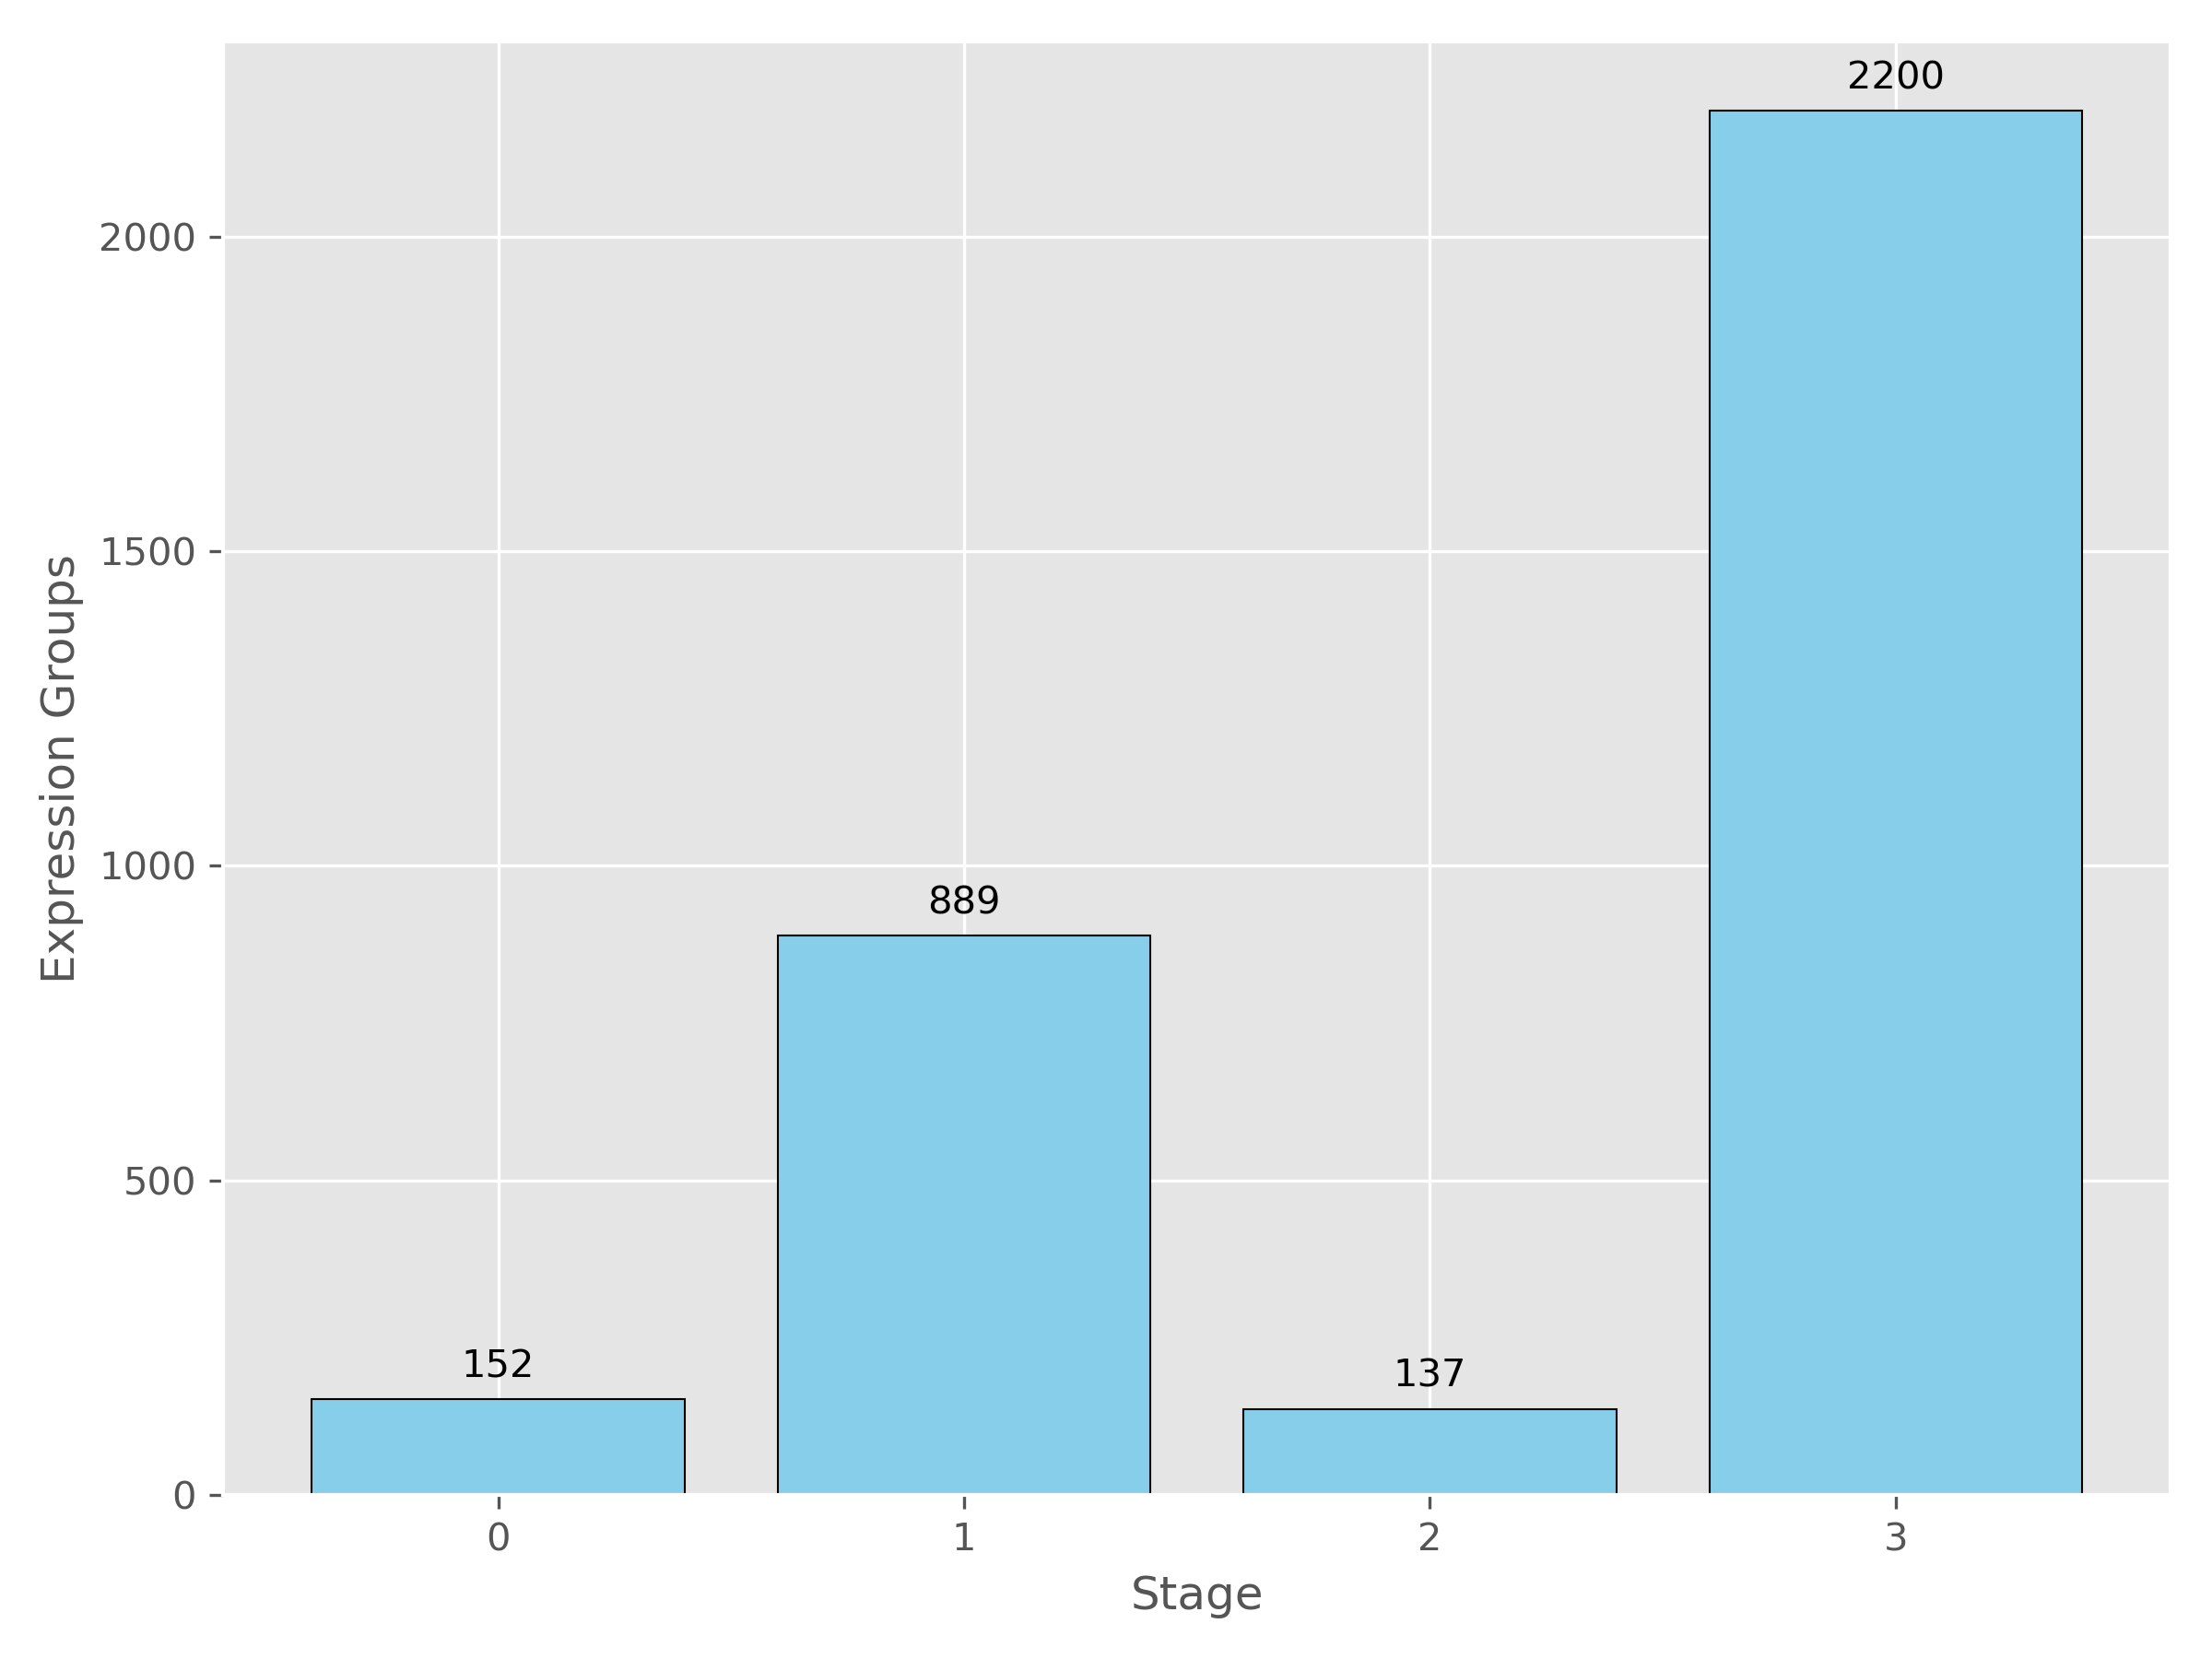
\includegraphics[width=0.80\linewidth]{img/expression_groups/q8_expression_groups.png}
    \caption{Query 8 - Expression Groups}
    \label{fig:exprgroups8}
\end{figure}
The histogram above displays the number of expression groups generated at each stage of the optimization process. Within each group, there may be an unknown number of equivalent expressions. \\
As we can see, the number of expression groups generated during stage 3 is significantly higher than in stage 2. This is a common pattern observed in the optimization process, where the optimizer explores a larger number of equivalent expressions in later stages. \\
This increase in expression groups is often accompanied by a decrease in the overall cost of the query, as the optimizer applies various transformations and optimizations to find more efficient execution plans. \\
This is also reflected in the histogram of cost reduction (Figure \ref{fig:cost1}), where we can see that the decrease in cost is more accentuated when we move from stage 2 to stage 3. \\
This is the stage where the optimizer applies the join reordering and hash join rules. \\

\subsection{Rule Application}

The rules set to be applied during stage 3 are the same as in \textbf{Query 2}, and they are defined in the \texttt{src/planner/rules/plan.rs} file. \\

\begin{figure}[H]
    \centering
    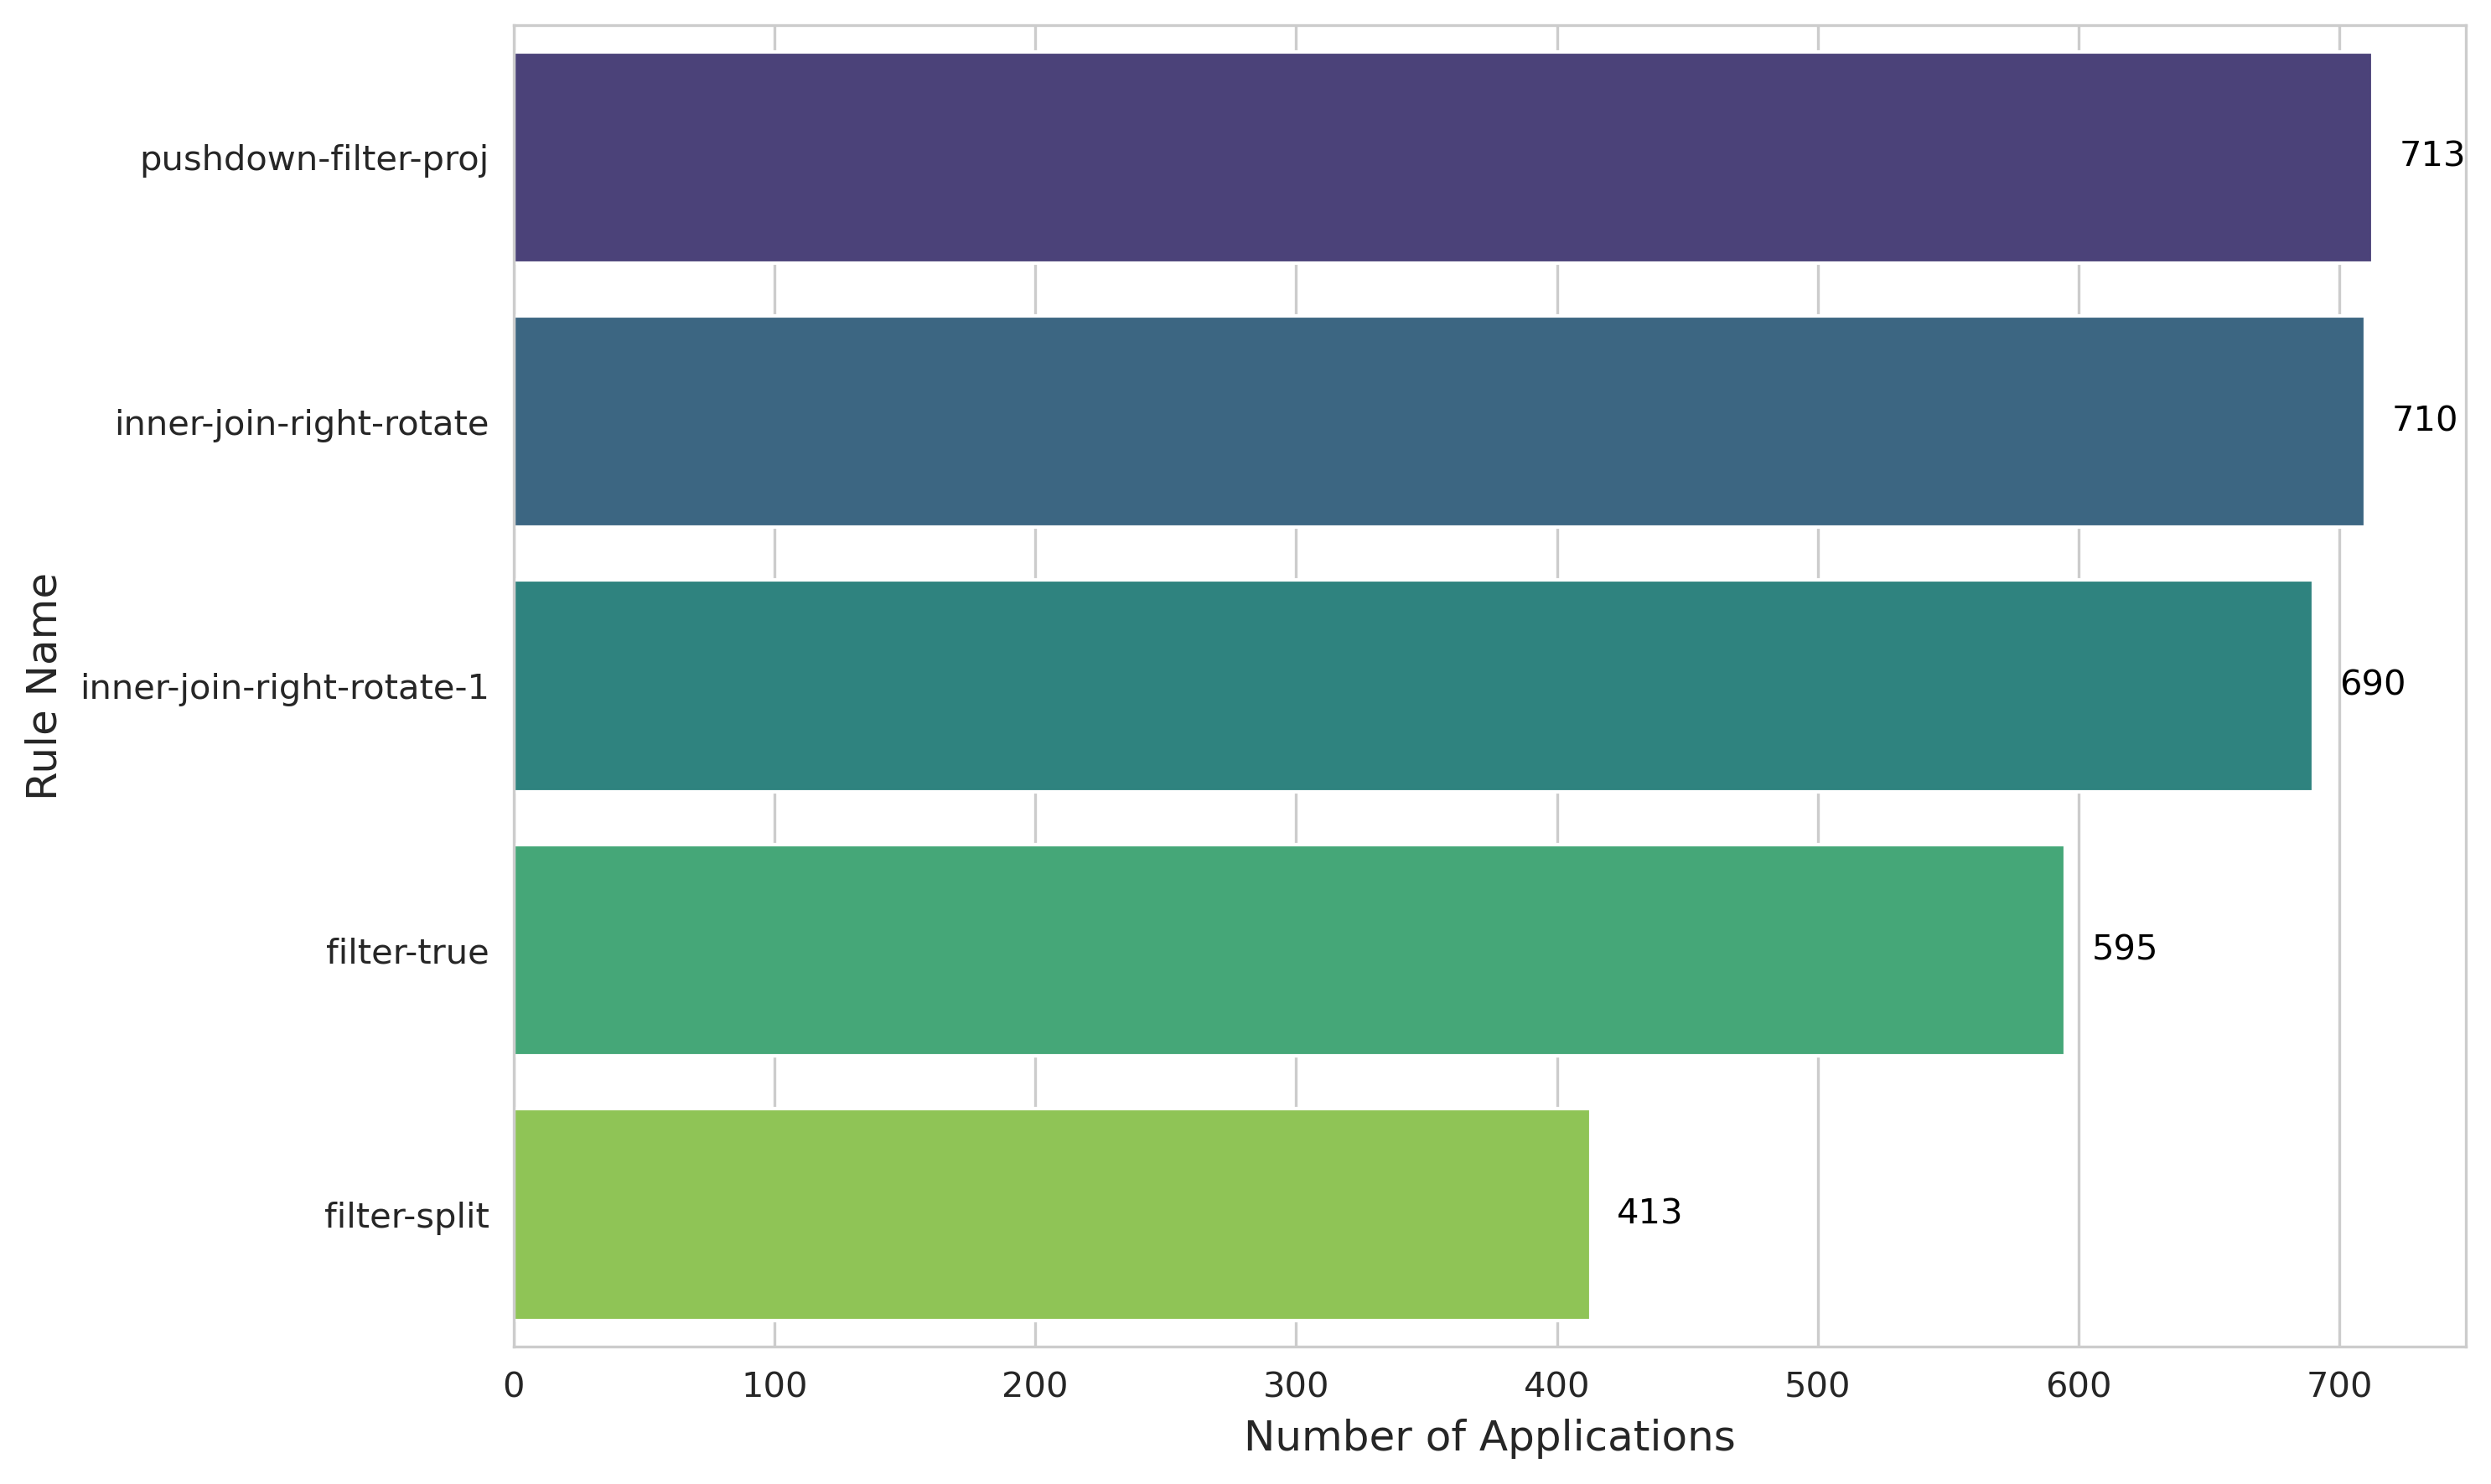
\includegraphics[width=0.95\linewidth]{img/img_rule_mostpop/top_5_rules_stage3_q8.png}
    \caption{Query 8 - Rules in Stage 3}
    \label{fig:rules8}
\end{figure}

The most frequently applied rules are related to join operations and projection pushdown. This aligns with our understanding that stage 3 focuses heavily on optimizing joins and their order of execution.
The high frequency of join-related rule applications explains the increase in expression groups, as each new join order or implementation strategy generates new equivalent expressions. Despite this increase in complexity, the optimizer successfully reduces the query's cost through these transformations.


\subsection{Merge Operations}
During stage 3, the optimizer applies join reordering rules and other transformations that generate a large number of new equivalent expressions. Each new join order or execution strategy can result in different representations for the same logical operation. As a consequence, the number of expression groups grows rapidly. \\

\begin{figure}[H]
    \centering
    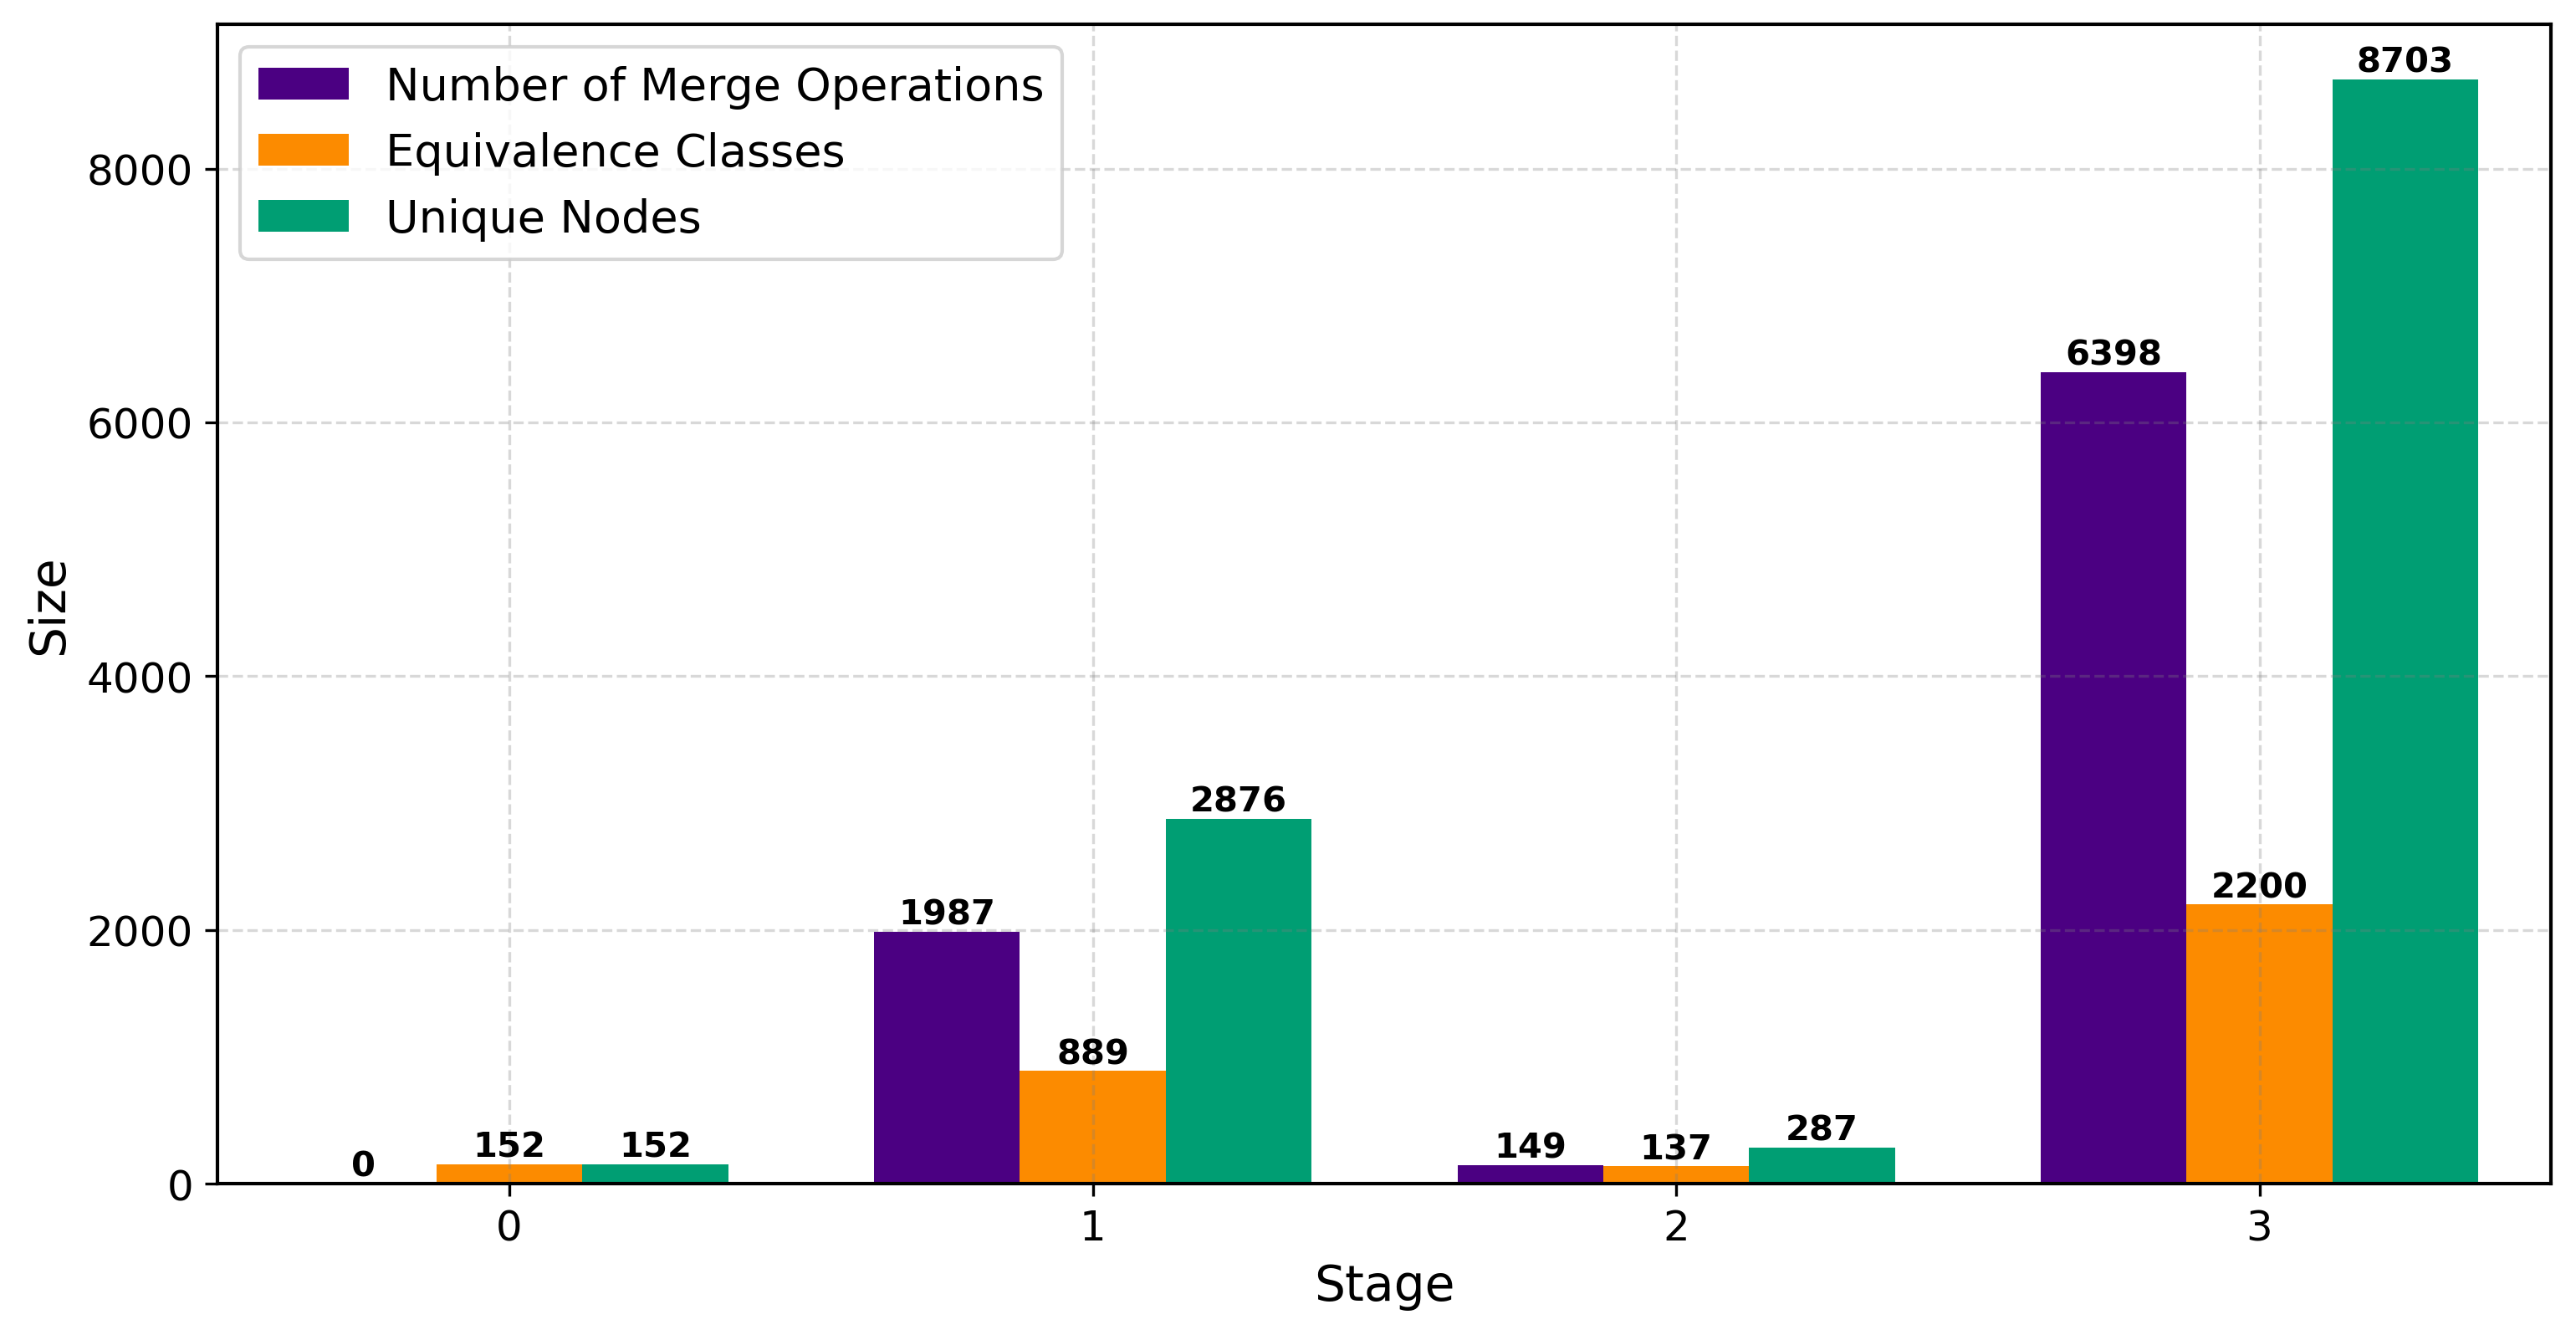
\includegraphics[width=\linewidth]{img_merges/q8_sizes.png}
    \caption{Query 8 - Merge operations}
    \label{fig:hist8}
\end{figure}




\chapter{Final Conclusions and Future Work} \label{chap:concl}
\thispagestyle{fancy}
This report describes our process of analyzing and visualizing the behavior of a SQL query optimizer through the instrumentation of the Risinglight database system. The project successfully achieved the objectives outlined in the introduction, providing valuable insights into the complex process of query optimization.

Our visual representations have made it possible to observe patterns and behaviors that would be difficult to discern from raw data alone. The analysis of expression groups, relational operators, and cost estimates has deepened our understanding of how different queries are optimized.

Some key findings from our analysis include:
\begin{itemize}
    \item The relationship between query complexity and the number of expression groups generated
    \item Common transformation patterns applied by the optimizer for specific query constructs
    \item Situations where cost estimates may not accurately reflect actual execution performance
\end{itemize}

While we believe that our project meets the requirements initially set, there is still room for future work. Potential extensions include:
\begin{itemize}
    \item Dynamic visualizations that show the step-by-step progression of the optimization process
    \item Interactive tools that allow users to modify queries and immediately see the impact on optimization
    \item Deeper analysis of specific optimization techniques, such as join reordering or predicate pushdown
    \item Integration with actual execution statistics to evaluate the effectiveness of optimization decisions
\end{itemize}

Overall, this project has provided valuable insights into query optimization and established a foundation for further research in this area.

\appendix

\chapter{Appendix}
\thispagestyle{fancy}

\section{README}

In order to run the project, you can make use of the \texttt{run.sh} script we developed to ease the analysis process. The README file in our GitHub Repository: \url{https://github.com/Blackparkd/risinglight/blob/main/README.md} contains all the necessary information to navigate the reader through this script. \\

\section{Important Links}
\begin{itemize}
    \item \textbf{Risinglight GitHub Repository:} \url{https://github.com/risinglightdb/risinglight}
    \item \textbf{Egg library:} \url{https://github.com/egraphs-good/egg}
    \item \textbf{Modified Risinglight GitHub Repository:} \url{https://github.com/Blackparkd/risinglight/tree/main}
    \item \textbf{Modified Egg library:} \url{https://github.com/Blackparkd/egg}
    \item \textbf{Generated histograms folder:} \url{https://github.com/Blackparkd/risinglight/tree/main/src/planner/outputs/graphs}
    \item \textbf{Python scripts:} \url{https://github.com/Blackparkd/risinglight/tree/main/src/planner/script}
    \item \textbf{Modified optimizer.rs file:} \url{https://github.com/Blackparkd/risinglight/blob/main/src/planner/optimizer.rs}
\end{itemize}

\section{References}
\begin{itemize}
    \item \textbf{Risinglight:} Risinglight is an open-source SQL database system designed for educational purposes. It is built on top of the Rust programming language and aims to provide high performance and scalability for data processing tasks.
    \item \textbf{Egg library:} Egg is a Rust library for writing and manipulating e-graphs. It provides a framework for implementing various optimization techniques, including those used in query optimization.
    \item \textbf{E-graphs:} E-graphs are data structures used to represent and optimize expressions in a way that allows for efficient manipulation and transformation. They are particularly useful in the context of query optimization, where multiple equivalent expressions may exist.
    \item \textbf{SQL:} SQL (Structured Query Language) is a standard programming language used for managing and manipulating relational databases. It allows users to perform various operations, such as querying data, inserting records, updating information, and deleting entries.
    \item \textbf{Query Optimization:} Query optimization is the process of transforming a SQL query into an efficient execution plan. It involves analyzing the query structure, applying various optimization techniques, and selecting the best plan based on cost estimates.
    \item \textbf{Relational Algebra:} Relational algebra is a formal system for manipulating relations (tables) in a database. It provides a set of operations, such as selection, projection, and join, that can be used to express queries and transformations on relational data.
    \item \textbf{TPC-H:} TPC-H is a widely used benchmark for evaluating the performance of database systems. It consists of a set of complex SQL queries that simulate real-world data processing scenarios, allowing researchers and developers to assess the efficiency of their systems.
    \item \textbf{Python:} Python is a high-level programming language known for its simplicity and readability. It is widely used for data analysis, visualization, and scripting tasks. In this project, Python was used to generate histograms and visualize the optimization process.
    \item \textbf{Matplotlib:} Matplotlib is a popular Python library for creating static, animated, and interactive visualizations. It provides a wide range of plotting functions and customization options, making it suitable for generating histograms and other types of charts.
    \item \textbf{Rust:} Rust is a systems programming language that emphasizes safety, concurrency, and performance. It is used in the Risinglight database system to implement the query optimizer and other components.
\end{itemize}

\section{Acknowledgments}
We would like to express our gratitude to Professor \textbf{José Orlando Pereira} for his guidance throughout this project. His expertise and insights were invaluable in shaping our understanding of query optimization and the Risinglight database system. \\
You can find more information about his work and research on his personal page:\\
\textbf{ \href{https://jopereira.github.io}{https://jopereira.github.io}}. \\


% Se precisares de glossário, ativa estas linhas:
% \usepackage{glossaries}
% \makeglossaries
% \printglossaries

\renewcommand{\headrulewidth}{0pt}

\end{document}
